
%----------------------------------------------------------------------------------------
%	CHAPTER 
%----------------------------------------------------------------------------------------
\chapterimage{chapter_head_cris1.pdf} % Chapter heading image

\chapter{ \Footwork~ no samba de gafieira }

Uma parte muito importante do desenvolvimento na dança é o treino e a repetição;
nesse sentido, o dançarino muitas vesses tem que investir em sim mesmo muito tempo 
de treinamento para desenvolver de forma fluida e natural seus movimentos.
Este é um trabalho duro e contínuo, que muitas vesses abordaremos de forma individual, 
e no nosso próprio tempo de aprendizagem; 
por isso é importante conhecer uma serie de exercícios que nos preparem,
fisicamente, e nos deem consciência corporal para executar nossos movimentos na dança.

Neste capítulo serão apresentados, uma serie de movimentos que podem ser usados,
no treinamento unipessoal; eles estão representados usando uma notação coreográfica
para o \footwork (do inglês ``footwork'' ) , que será previamente explicada.
 
\section{Notação coreográfica para o \footwork }
Para descrever o \footwork~ numa representação escrita, 
será usado uma notação baseada numa vista da posição dos pés no chão. 
Existirá uma representação para cada subdivisão temporal do movimento, 
estas subdivisões serão chamadas de tempos coreográficos, 
para diferenciar-lhos dos tempos do compasso; 
pois a duração e o inicio destos será diferente\footnote{Para 
mais detalhes da contagem dos tempos no compasso, ver Seção \ref{sec:Tempo}.}.

A Tabela \ref{tab:notationunipessoal} descreve o significado de todos os símbolos usados,
na notação coreográfica para o \footwork.
\begin{longtable}{| c |p{0.80\textwidth}  |}
  %\begin{tabular}{| p{0.1\textwidth}|p{0.80\textwidth}  |}
  \hline
  Símbolo & Descrição \\ \hline \hline 
  T & Abreviatura do termo \textbf{tempo}, se referindo ao tempo do compasso na música, ver Seção \ref{sec:Tempo}. \\ \hline

  TC & Abreviatura do termo \textbf{tempo coreográfico}, 
  de modo que cada movimento é subdividido temporalmente num número de TC. 
  Todos os TC são definidos na descrição de cada movimento, 
  tendo sempre neste âmbito a mesma duração;
  porem, este é um valor relativo ao tempo musical, e cada movimento pode usar um TC de 1, 1/2 ou 1/4 do tempo musical,
  procurando otimizar a didática na explicação do movimento. \\ \hline

  \raisebox{-\totalheight}{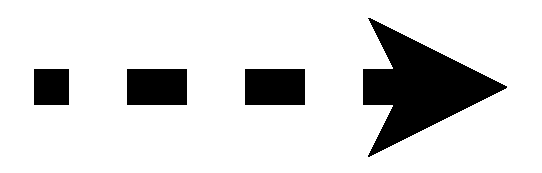
\includegraphics[width=1cm]{notation-foot/notacion1-seta.eps}} & A \textbf{seta} 
  indica o percorrido para que um pé chegue à posição do TC atual; é dizer, nos fala do passado do TC.
  A cor pode variar em função se no final do movimento se chega com o peso do corpo. \\ \hline 

  \raisebox{-\totalheight}{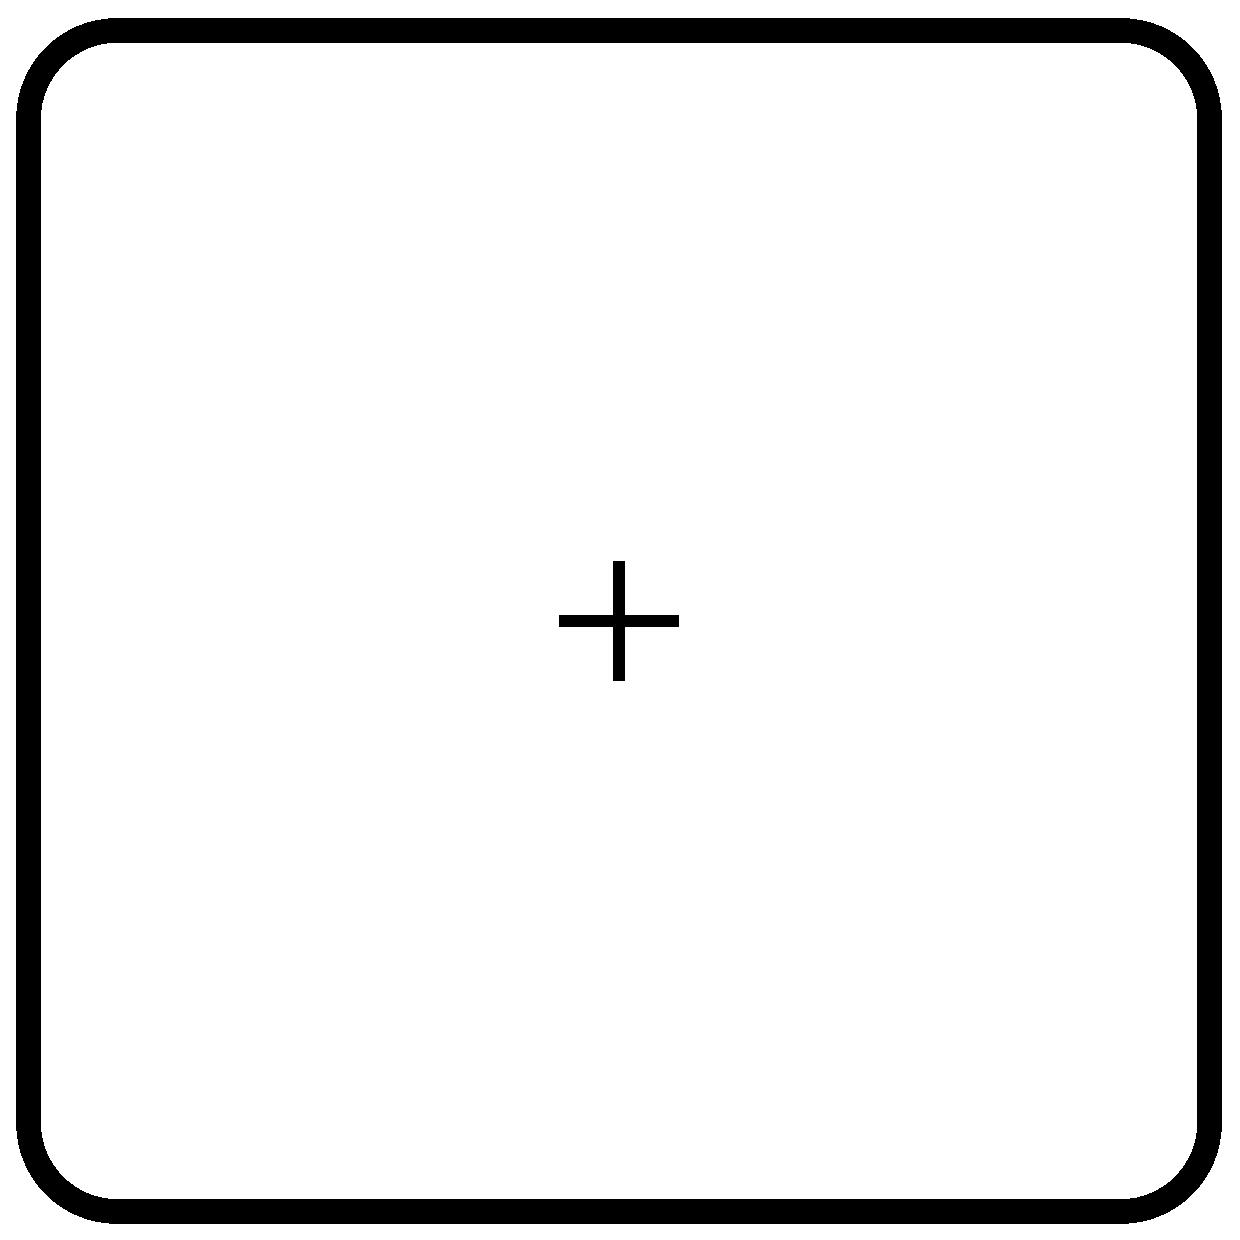
\includegraphics[width=1cm]{notation-foot/notacion-box.eps}} & 
  O \textbf{quadro de trabalho} é onde se colocará a disposição dos pés no chão, em cada tempo coreográfico,
  de modo que esta disposição indica o estado no inicio do TC.  \\ \hline
  %Se consideramos ao \textbf{quadro de trabalho} um plano cartesiano a posição (0,0) é indicado com um símbolo de +.  \\ \hline

  \raisebox{-\totalheight}{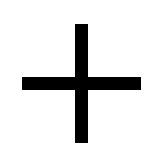
\includegraphics[width=0.4cm]{notation-foot/notacion-plus.eps}} & 
  Este símbolo indica a \textbf{origem} ou posição (0,0), do plano cartesiano que representa o \textbf{quadro de trabalho};
  e pode ser colocado em qualquer lugar deste. \\ \hline

  \raisebox{-\totalheight}{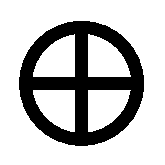
\includegraphics[width=0.4cm]{notation-foot/notacion-plusc.eps}} & 
  Este símbolo indica a posição da \textbf{próxima origem} ou posição (0,0), 
  do plano cartesiano que representa \textbf{quadro de trabalho};
  isto será usado para descrever movimentos com deslocamentos longos.
  Este símbolo pode ser colocado em qualquer lugar do \textbf{quadro de trabalho}. \\ \hline

  \raisebox{-\totalheight}{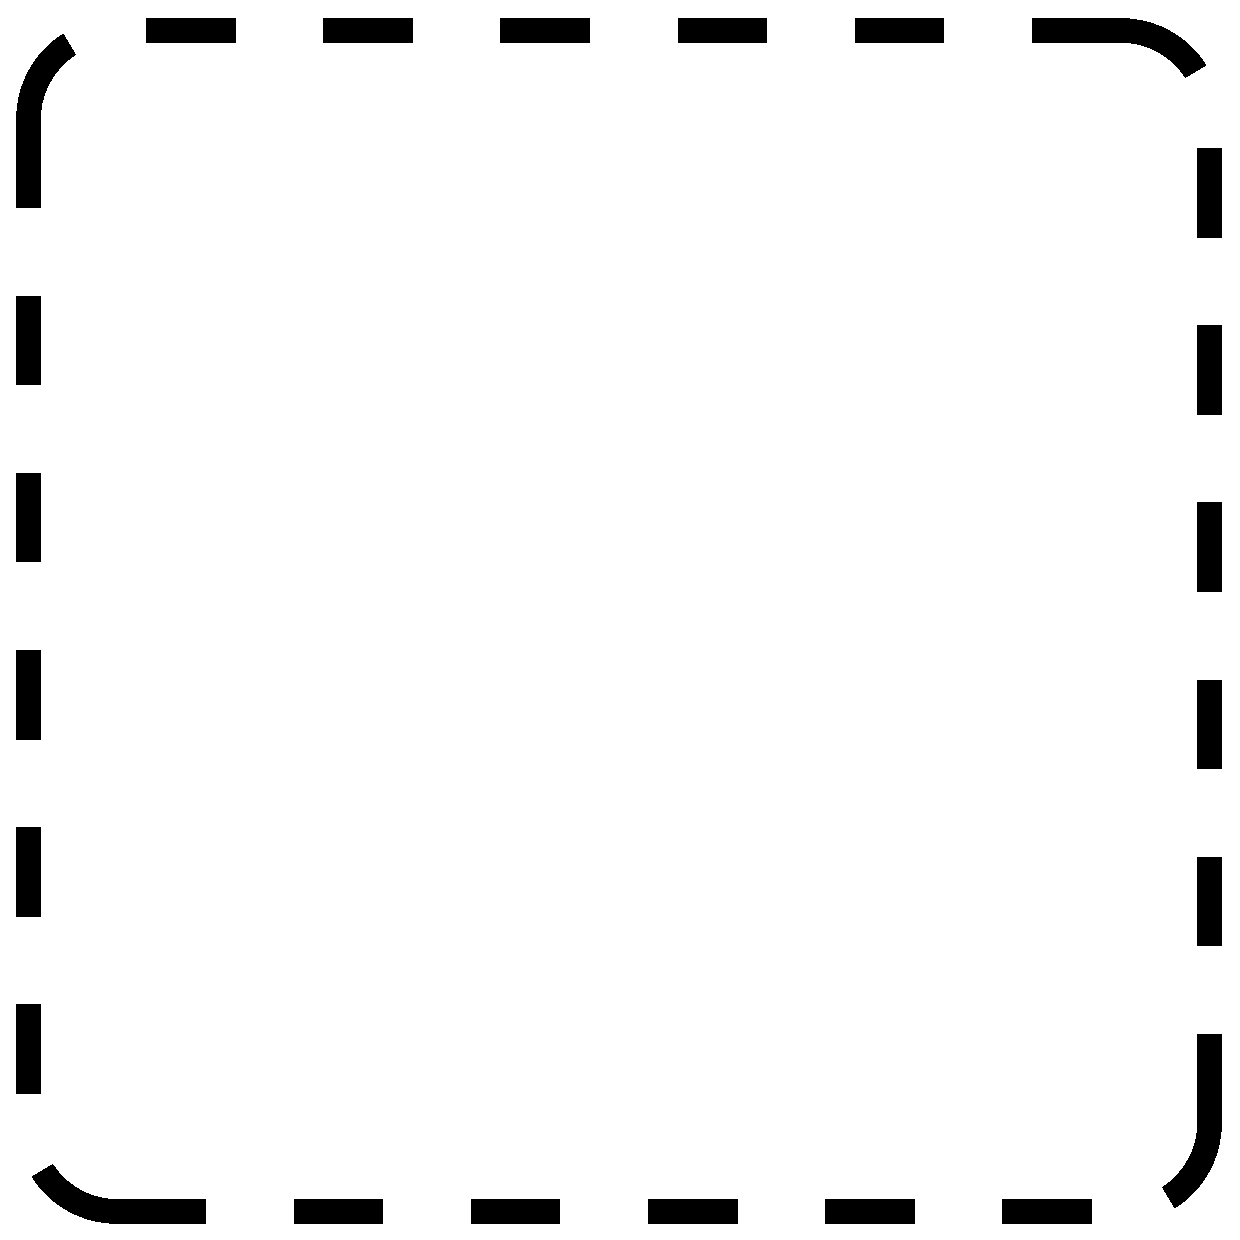
\includegraphics[width=1cm]{notation-foot/notacion-box-dot.eps}} & 
  O \textbf{quadro de descanso} é um símbolo que indica que nesse tempo coreográfico não se realizará movimento de pés;
  desenhar este quadro é opcional, dado que se entende que se o quadro não está desenhado então não existe informação 
  de movimento nesse tempo, o único proposito é didático para melhorar a clareza das representações.  \\ \hline


  \raisebox{-\totalheight}{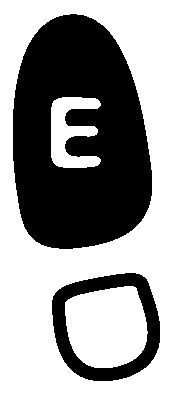
\includegraphics[height=1.2cm]{notation-foot/notacion-esq-preto.eps}} & Este símbolo 
  indica o \textbf{pé esquerdo}; 
  o calcanhar está desenhado com branco para indicar que essa parte do pé não deve suportar 
  o peso do corpo.
  A cor da parte dianteira do pé pode variar em função se este tiver o peso do corpo. \\ \hline  

  \raisebox{-\totalheight}{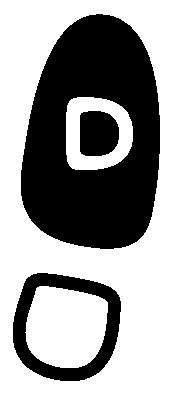
\includegraphics[height=1.2cm]{notation-foot/notacion-der-preto.eps}} & Este símbolo 
  indica o \textbf{pé direito}; 
  o calcanhar está desenhado com branco para indicar que essa parte do pé não deve suportar 
  o peso do corpo. 
  A cor da parte dianteira do pé pode variar em função se este tiver o peso do corpo. \\ \hline  

  \raisebox{-\totalheight}{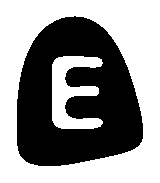
\includegraphics[height=0.6cm]{notation-foot/notacion-esq-preto-ponta.eps}} & Este símbolo 
  indica que se usará a \textbf{ponta do pé esquerdo};
  a porção da ponta que será usada quedará a decisão de cada dançarino. 
  A cor pode variar em função se este pé tiver o peso do corpo. \\ \hline  

  \raisebox{-\totalheight}{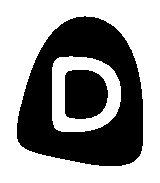
\includegraphics[height=0.60cm]{notation-foot/notacion-der-preto-ponta.eps}} & Este símbolo 
  indica que se usará a \textbf{ponta do pé direito};
  a porção da ponta que será usada quedará a decisão de cada dançarino. 
  A cor pode variar em função se este pé tiver o peso do corpo. \\ \hline


  \raisebox{-\totalheight}{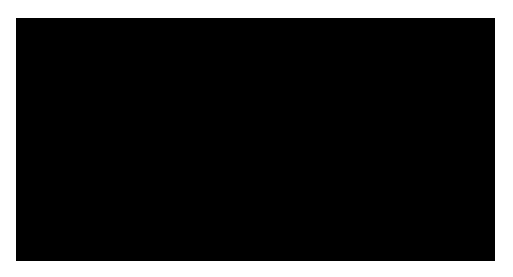
\includegraphics[width=1cm]{notation-foot/notacion-preto.eps}} & Os símbolos 
  com esta cor indicam que o pé ao que fazem referencia \textbf{tem o peso do corpo}. \\ \hline 

  \raisebox{-\totalheight}{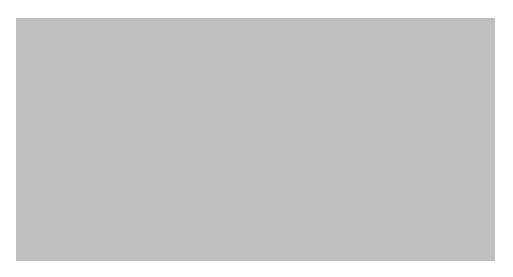
\includegraphics[width=1cm]{notation-foot/notacion-gris.eps}} & Os símbolos 
  com esta cor indicam que o pé ao que fazem referencia \textbf{não tem o peso do corpo}. \\ \hline

  \raisebox{-\totalheight}{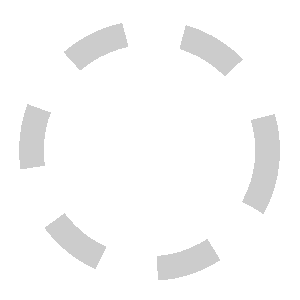
\includegraphics[width=1cm]{notation-foot/notacion-pica-pau.eps}} & 
  O símbolo \textbf{pica-pau} indica que não existe deslocamento e só levantaremos o pé
  e o colocaremos no mesmo lugar, este simbolo é usado quando esse pé não tem o peso do corpo.  \\ \hline

  \raisebox{-\totalheight}{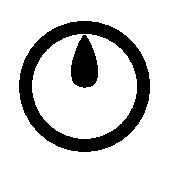
\includegraphics[width=1cm]{notation-foot/notacion-quadril.eps}} & 
  A \textbf{buzula} indica um vetor paralelo à direção onde deve apontar o quadril.
  O uso deste símbolo é opcional, e só é usado quando a informação do quadril é relevante
  para o exercício.   \\ \hline


  \raisebox{-\totalheight}{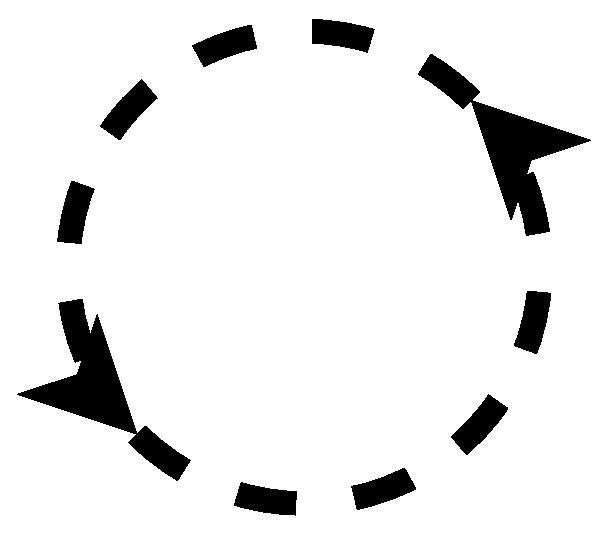
\includegraphics[width=1cm]{notation-foot/notacion-twist-antihorario.eps}} & 
  O símbolo indica um \textbf{twist} com o pé em sentido antihorário. \\ \hline 

  \raisebox{-\totalheight}{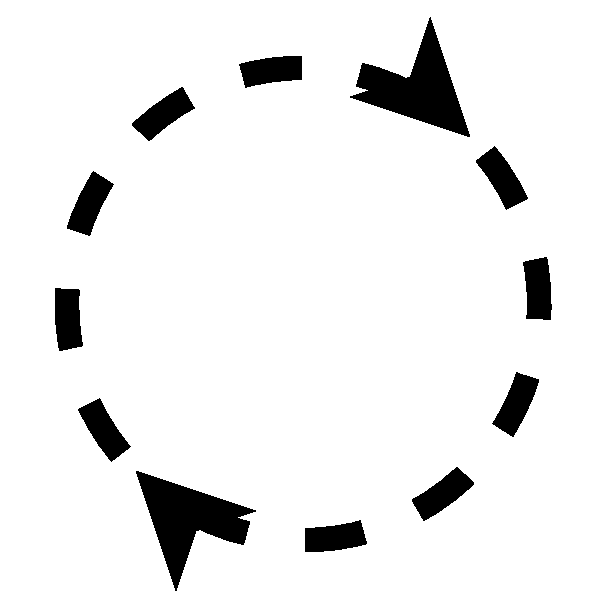
\includegraphics[width=1cm]{notation-foot/notacion-twist-horario.eps}} & 
  O símbolo indica um \textbf{twist} com o pé em sentido horário. \\ \hline

  %\end{tabular}
  \caption{Notação coreográfica para o \footwork.}
  \label{tab:notationunipessoal}
\end{longtable}

%\section{\textcolor{blue}{Movimentos para trabalhar de forma individual}}

Nas seguintes seções serão descritos uma serie de movimentos que poderão ser treinados individualmente.
Estes são interessantes para o desenvolvimento de consciência corporal, 
e poderão ser usados posteriormente na dança a dois,
fazendo algumas leves modificações ou adaptações.\\

\begin{tcbattention}
Nas seguintes seções, é usado o termo \textbf{variante} para descrever aos movimentos;
devido a que para cada movimento, na dança, 
existe uma grande variedade de formas ou estilos de realizar estes.
Assim, é difícil estabelecer um critério comum para apontar a forma oficial para a realização de cada movimento,
pelo que estes serão referenciados sempre como variantes. 
\end{tcbattention}

%%%%%%%%%%%%%%%%%%%%%%%%%%%%%%%%%%%%%%%%%%%%%%%%%%%%%%%%%%%%%%%%%%%%%%%%%%%%%%%%
\clearpage
\section{ \Variante: Trança}
\index{Passo!Trança}

A Figura \ref{fig:pessoaltranca} mostra os movimentos necessários para executar uma variante do passo chamado trança.
\begin{itemize}
\item Cada quadro de trabalho representa a posição dos pés em cada tempo coreográfico;
\item um tempo coreográfico tem uma duração igual a meio tempo musical.
\item A trança é um movimento que pode ser executado de forma cíclica, de modo que 
a sequencia de passos pode executar-se como: TC1, TC2, ..., TC7, TC8, TC1, ..., etc.  
Quantas vesses se considere necessário.
\end{itemize}
\begin{figure}[!h]
  \centering
    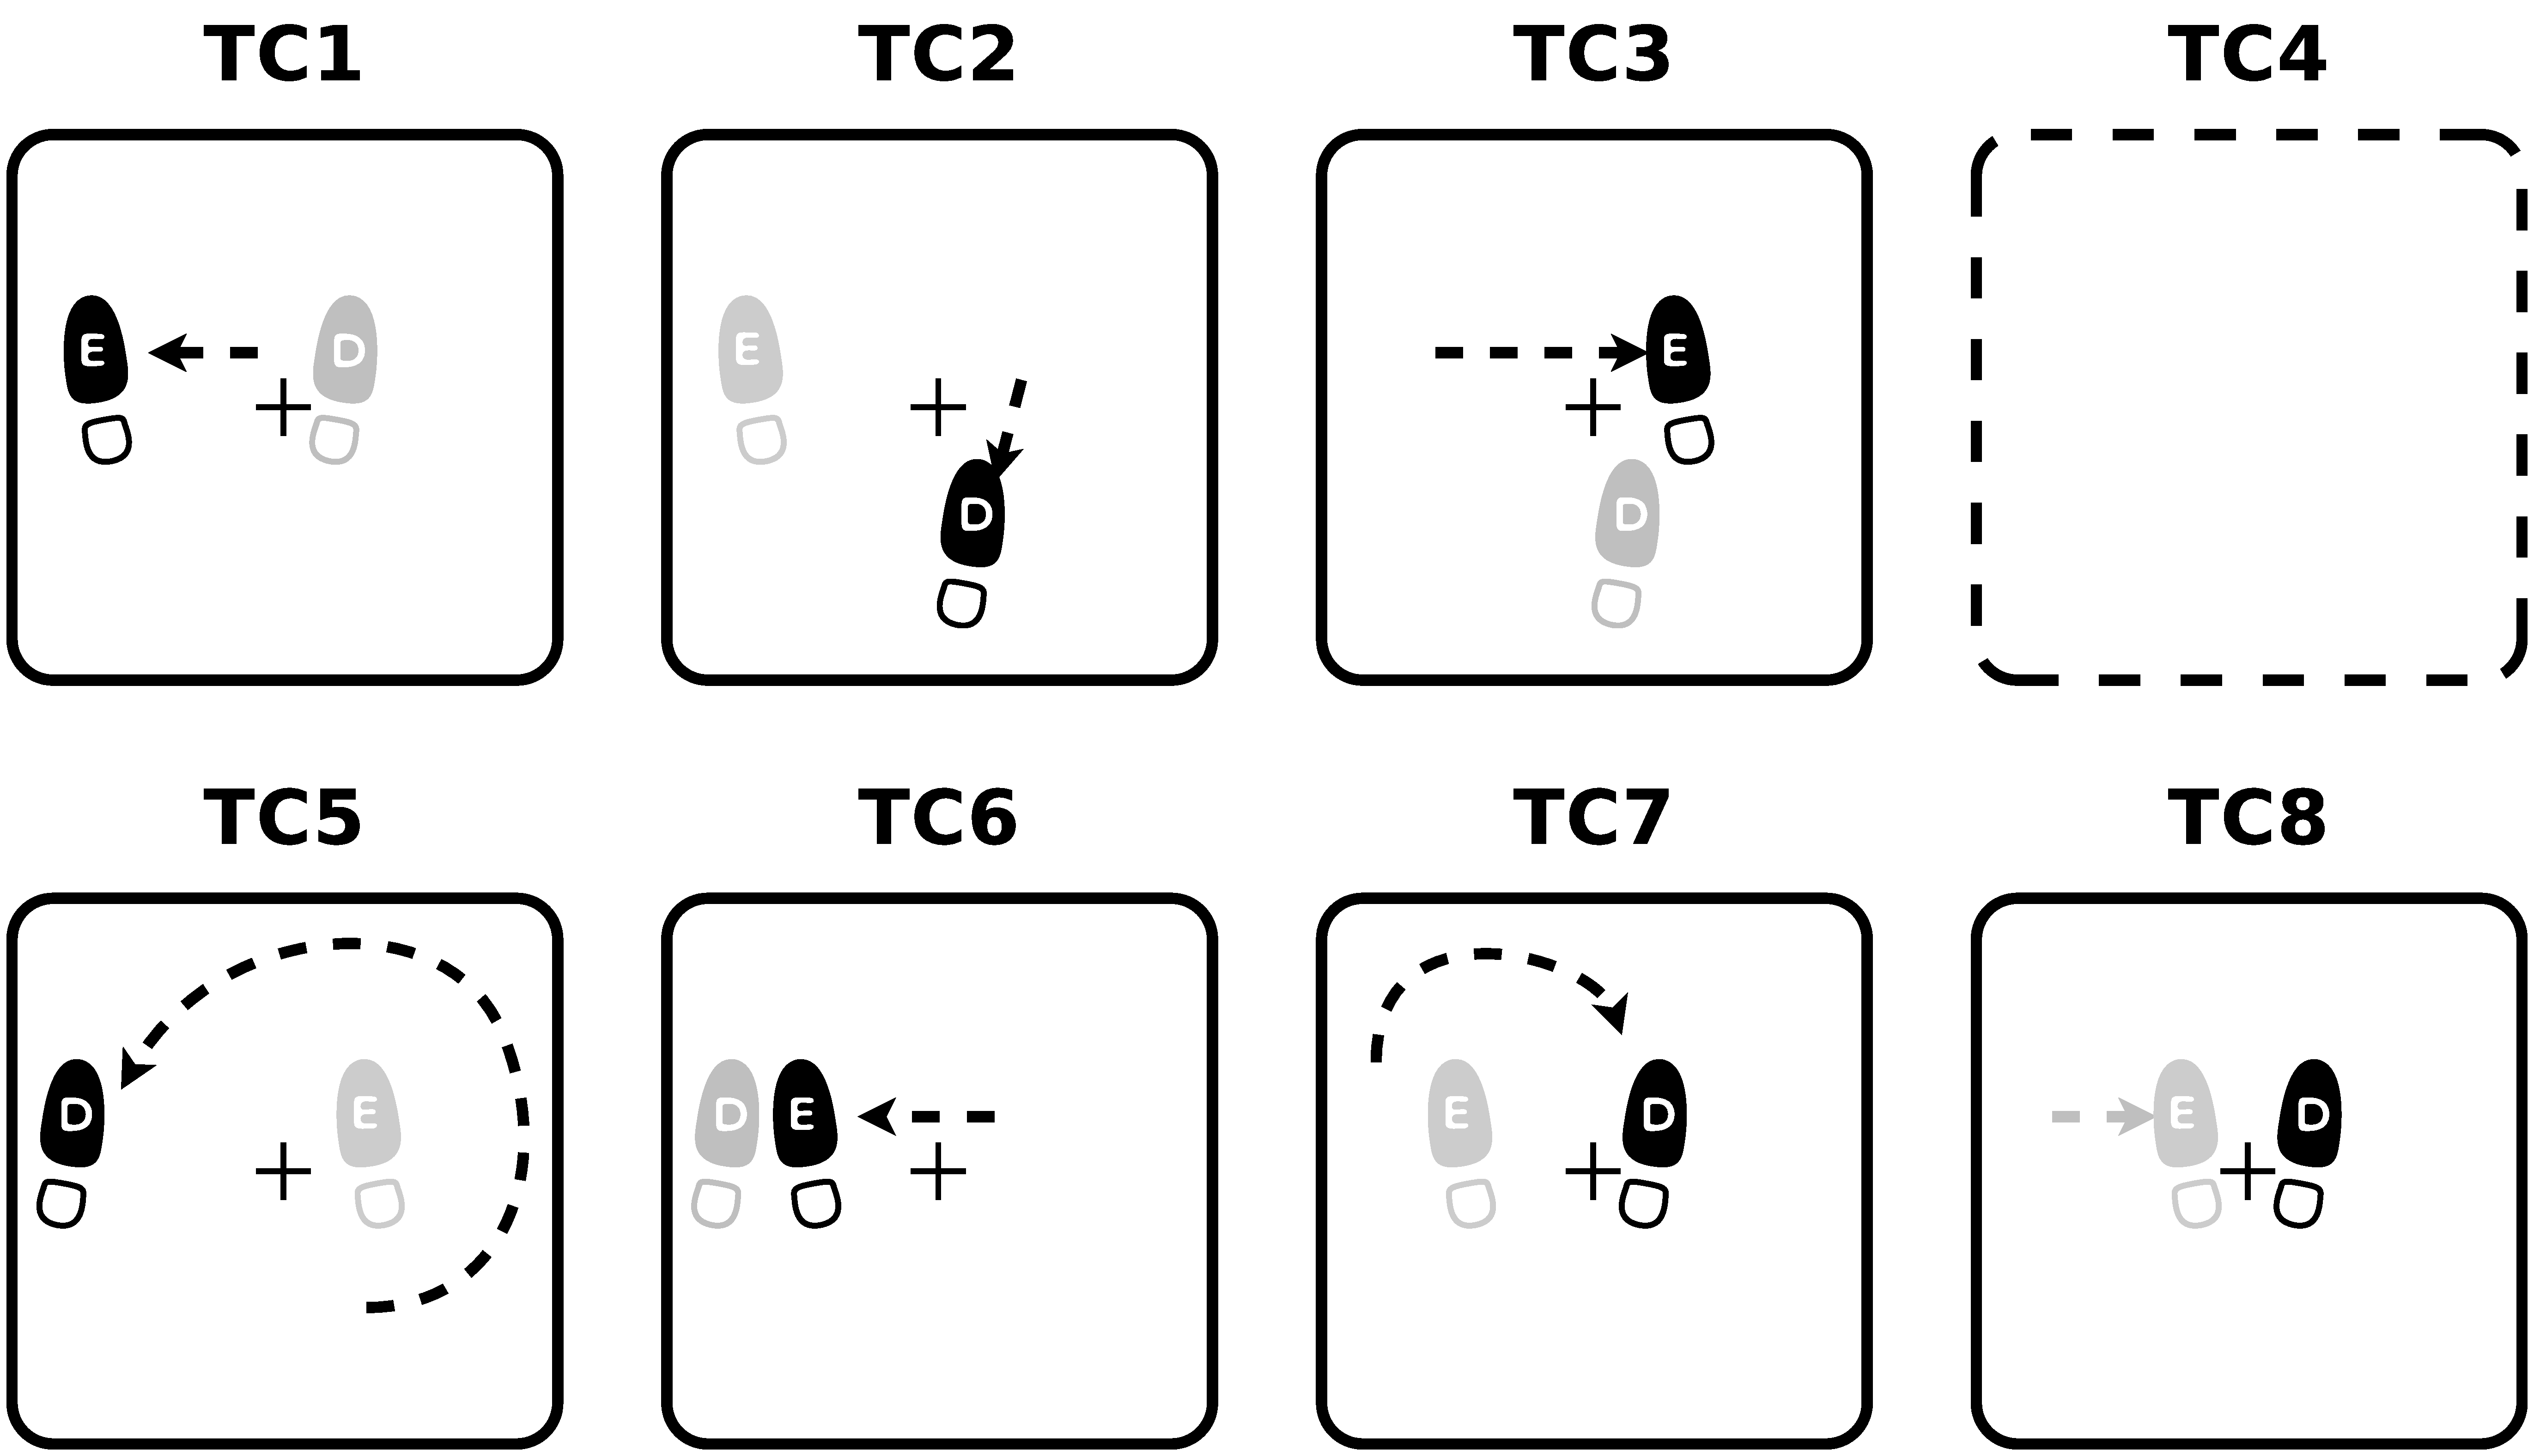
\includegraphics[width=\workboxsize]{chapters/cap-passos-footwork/tranca.eps}
\caption{Diagrama de tempos coreográficos para a trança, $T=2~TC$.}
\label{fig:pessoaltranca}
\end{figure}

A Figura \ref{fig:abc-pessoaltrancatc2} mostra o diagrama de tempos para realizar o movimento trança,
iniciando com o tempo forte da música.
\begin{figure}[!h]
  \centering
\begin{abc}[name=abc-pessoaltrancatc2,width=0.7\linewidth]
X: 1 % start of header
K: C stafflines=1 % scale: C major
M: 2/4 %meter - compasso
%Q:1/4=80
V:1 clef=perc stem=up name="Ritmo" sname="Ritmo"
V:2 clef=perc stem=up name="TC"    sname="TC"
[V:1] |: B2  B1  B1 | B2  B1  B1 :| 
w:       tum  tchic tchic tum tchic tchic 
w: ~ ~ ~ ~ ~ ~ 
%w: ~ ~ ~ ~ ~ ~ 
[V:2] |: B1  B1  B2   | B1 B1  B1  B1 :| 
w:       TC1 TC2  TC3   TC5 TC6 TC7 TC8
\end{abc}
\caption{Diagrama de tempos para a execução da trança.}
\label{fig:abc-pessoaltrancatc2}
\end{figure}

Dependendo do movimento ou passo, desde onde entremos na trança, 
em alguns momentos faremos este movimento iniciando desde o tempo fraco da música; 
nesse contexto, a Figura \ref{fig:abc-pessoaltranca} mostra a distribuição de tempos para realizar 
este movimento.
\begin{figure}[!h]
  \centering
\begin{abc}[name=abc-pessoaltranca,width=0.7\linewidth]
X: 1 % start of header
K: C stafflines=1 % scale: C major
M: 2/4 %meter - compasso
%Q:1/4=80
V:1 clef=perc stem=up name="Ritmo" sname="Ritmo"
V:2 clef=perc stem=up name="TC"    sname="TC"
[V:1] |: B2  B1  B1 | B2  B1  B1 :| 
w:       ~   tchic tchic tum tchic tchic 
w:       tum ~     ~     ~   ~     ~    
w: ~ ~ ~ ~ ~ ~ 
%w: ~ ~ ~ ~ ~ ~ 
[V:2] |: B1  B1  B1  B1 | B2  B1  B1 :| 
w:       ~   ~   TC1 TC2  TC3 TC5 TC6 
%w:       ~ ~ ~ ~   ~ ~ ~ ~ 
w:       TC7 TC8  ~  ~    ~       ~   ~    
\end{abc}
\caption{Diagrama de tempos para a execução da trança.}
\label{fig:abc-pessoaltranca}
\end{figure}

%%%%%%%%%%%%%%%%%%%%%%%%%%%%%%%%%%%%%%%%%%%%%%%%%%%%%%%%%%%%%%%%%%%%%%%%%%%%%%%%
\clearpage
\section{\Variante: Samba no pé}\index{Passo!Samba no pé}

A Figura \ref{fig:pessoa-samba-no-pe} mostra os movimentos necessários para executar uma variante do passo de samba no pé para atrás.
\begin{itemize}
\item Cada quadro de trabalho representa a posição dos pés em cada tempo coreográfico;
\item um tempo coreográfico tem uma duração igual a meio tempo musical (T).
\item O passo básico de samba no pé  pode ser executado de forma cíclica, de modo que 
a sequencia de passos pode executar-se como: TC1, TC2, ..., TC7, TC8, TC1, ..., etc.  
Quantas vesses se considere necessário.
\end{itemize}
\begin{figure}[!h]
  \centering
    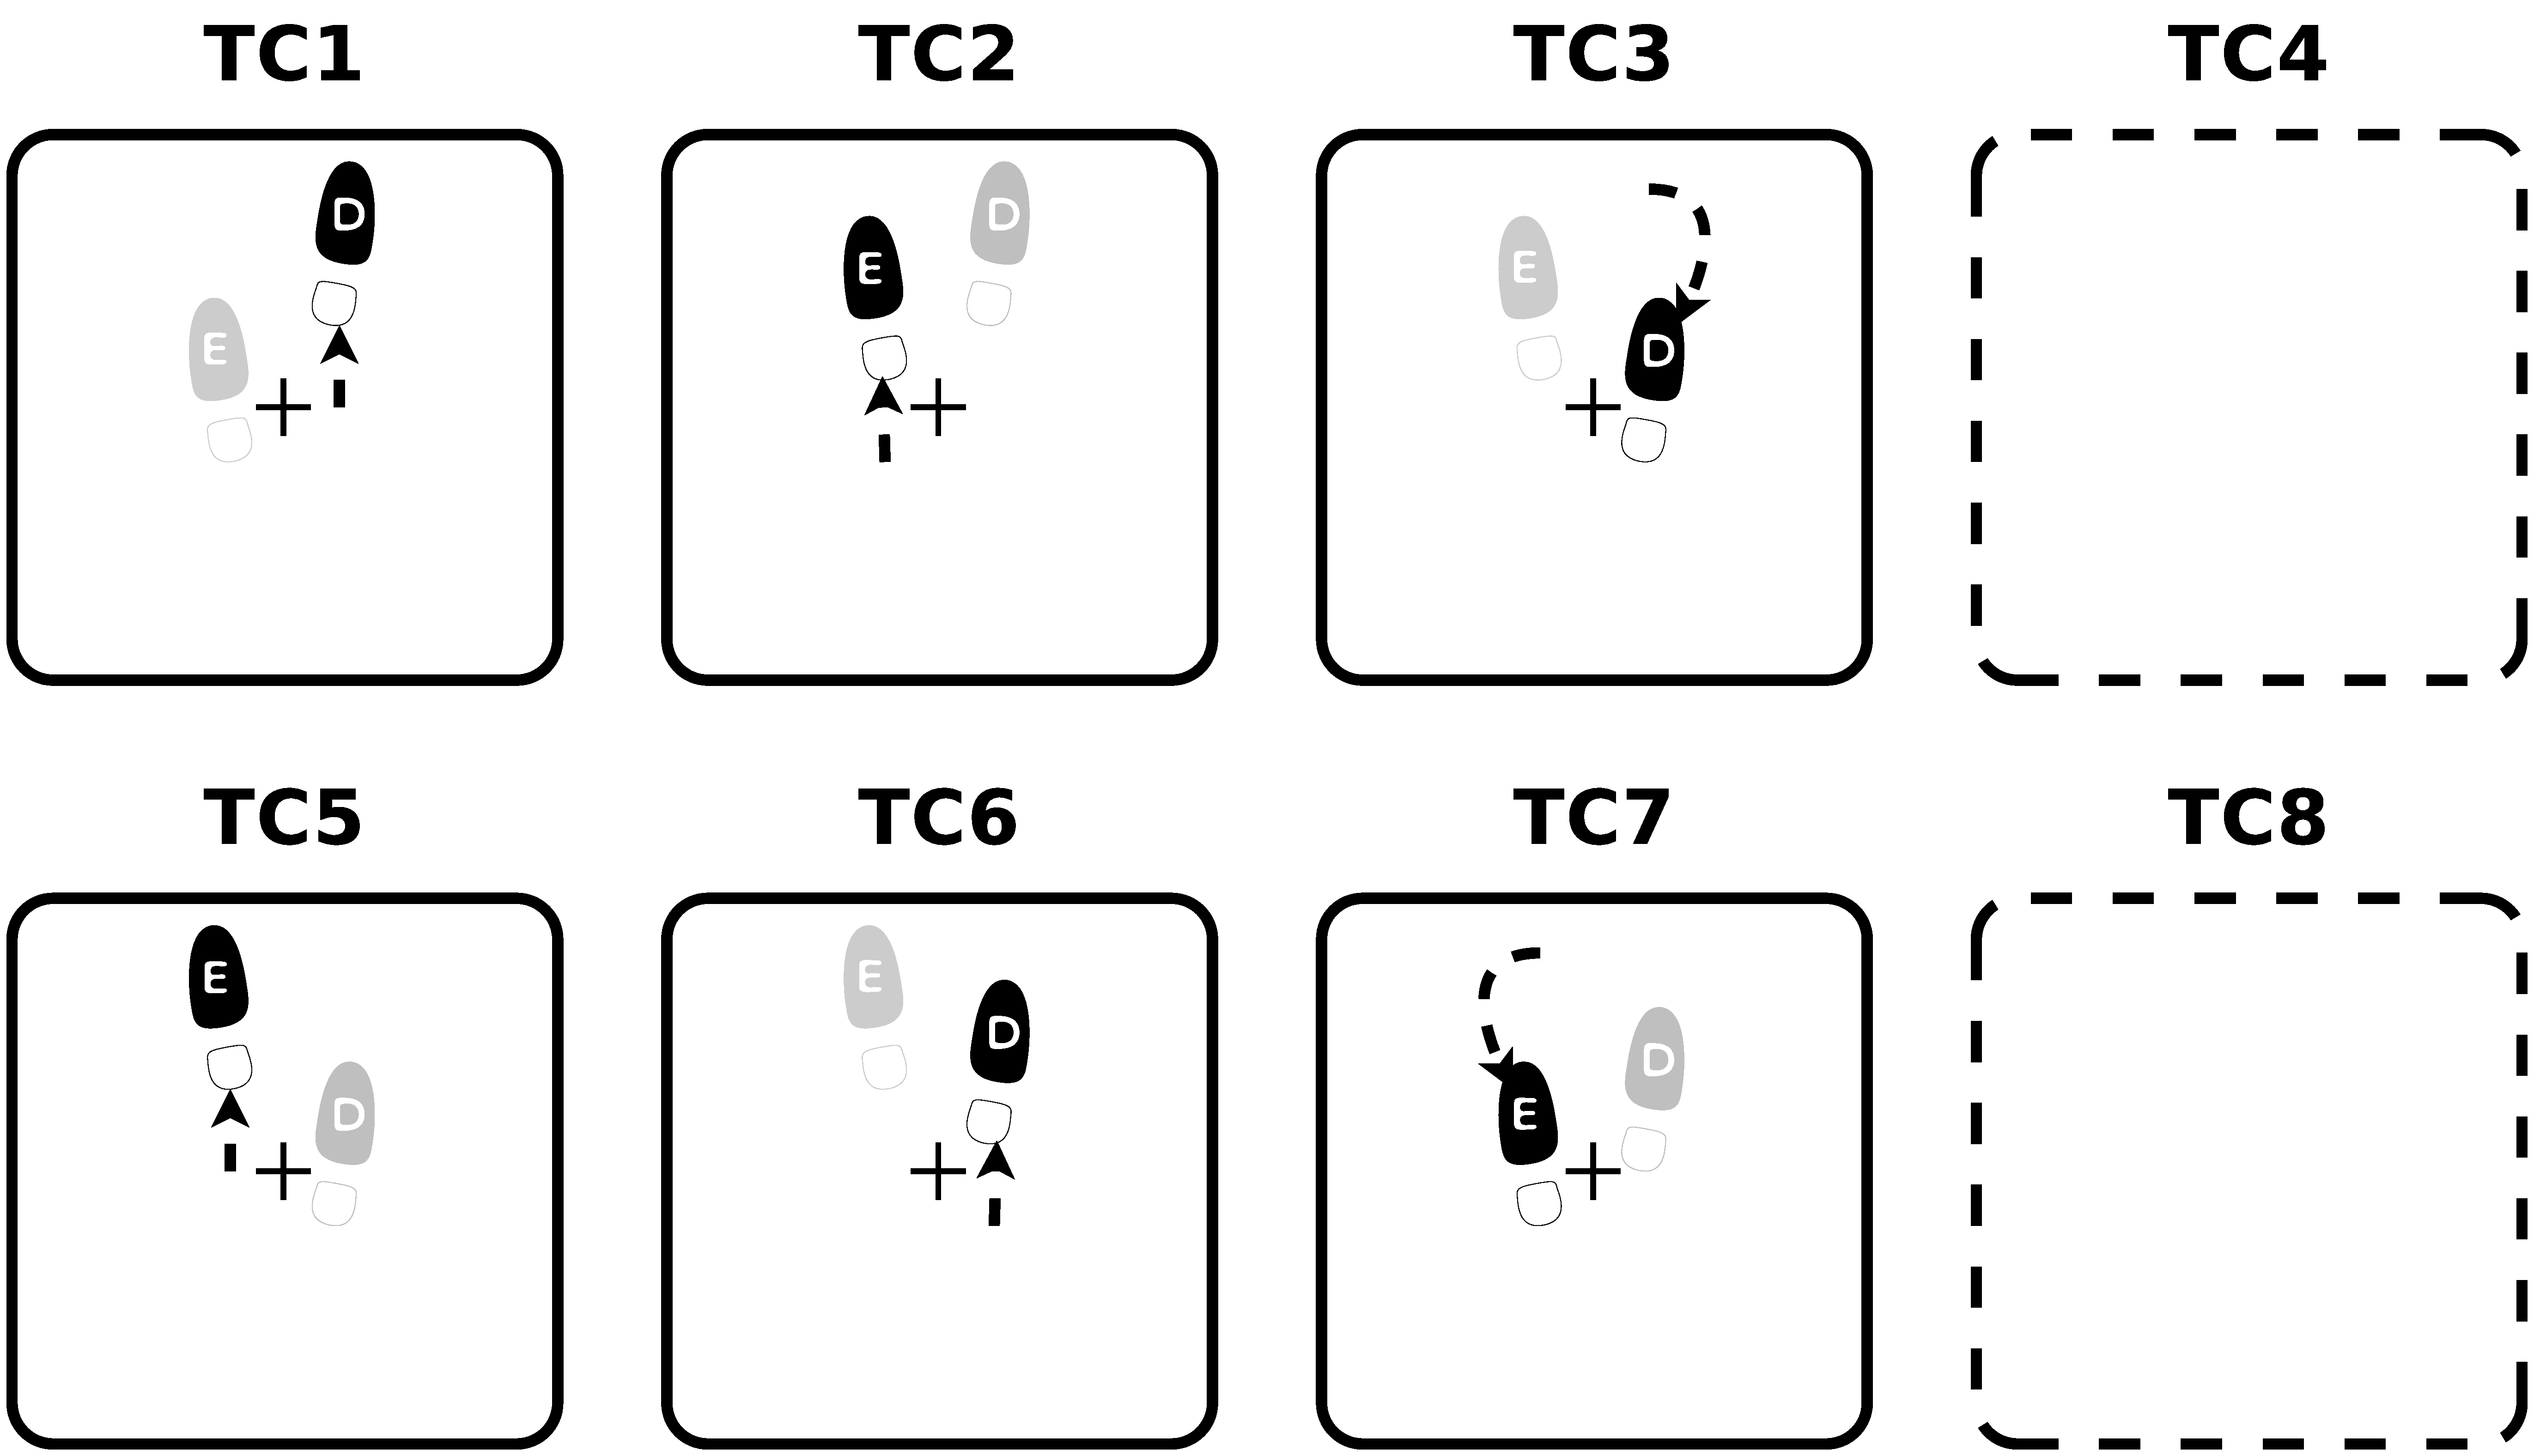
\includegraphics[width=\workboxsize]{chapters/cap-passos-footwork/samba-no-pe.eps}
\caption{Diagrama de tempos coreográficos para o passo de samba no pé  para atrás, $T=2~TC$.}
\label{fig:pessoa-samba-no-pe}
\end{figure}


A Figura \ref{fig:abc-pessoalsambape1} mostra o diagrama de tempos coreográficos para realizar o passo de samba no pé,
pra adiante.
\begin{figure}[!h]
  \centering
\begin{abc}[name=abc-pessoalsambape1,width=0.7\linewidth]
X: 1 % start of header
K: C stafflines=1 % scale: C major
M: 2/4 %meter - compasso
%Q:1/4=80
V:1 clef=perc stem=up name="Ritmo" sname="Ritmo"
V:2 clef=perc stem=up name="TC"    sname="TC"
[V:1] |: B2  B1  B1 | B2  B1  B1 :| 
w:       ~  tchic tchic tum tchic tchic 
w: tum ~ ~ ~ ~ ~ 
w: ~ ~ ~ ~ ~ ~ 
[V:2] |: B2  B1  B1 | B2  B1  B1 :| 
w:       ~   TC1 TC2  TC3 TC5 TC6 
w:       TC7  
\end{abc}
\caption{Diagrama de tempos para a execução do passo do samba no pé para atrás.}
\label{fig:abc-pessoalsambape1}
\end{figure}

%%%%%%%%%%%%%%%%%%%%%%%%%%%%%%%%%%%%%%%%%%%%%%%%%%%%%%%%%%%%%%%%%%%%%%%%%%%%%%%%
\clearpage
\section{\Variante~2: Samba no pé}\index{Passo!Samba no pé}

A Figura \ref{fig:pessoa-samba-no-pe-b} mostra os movimentos necessários para executar uma variante do passo de samba no pé para atrás.
\begin{itemize}
\item Cada quadro de trabalho representa a posição dos pés em cada tempo coreográfico;
\item um tempo coreográfico tem uma duração igual a meio tempo musical (T).
\item O passo básico de samba no pé  pode ser executado de forma cíclica, de modo que 
a sequencia de passos pode executar-se como: TC1, TC2, ..., TC7, TC8, TC1, ..., etc.  
Quantas vesses se considere necessário.
\end{itemize}

\begin{figure}[!h]
  \centering
    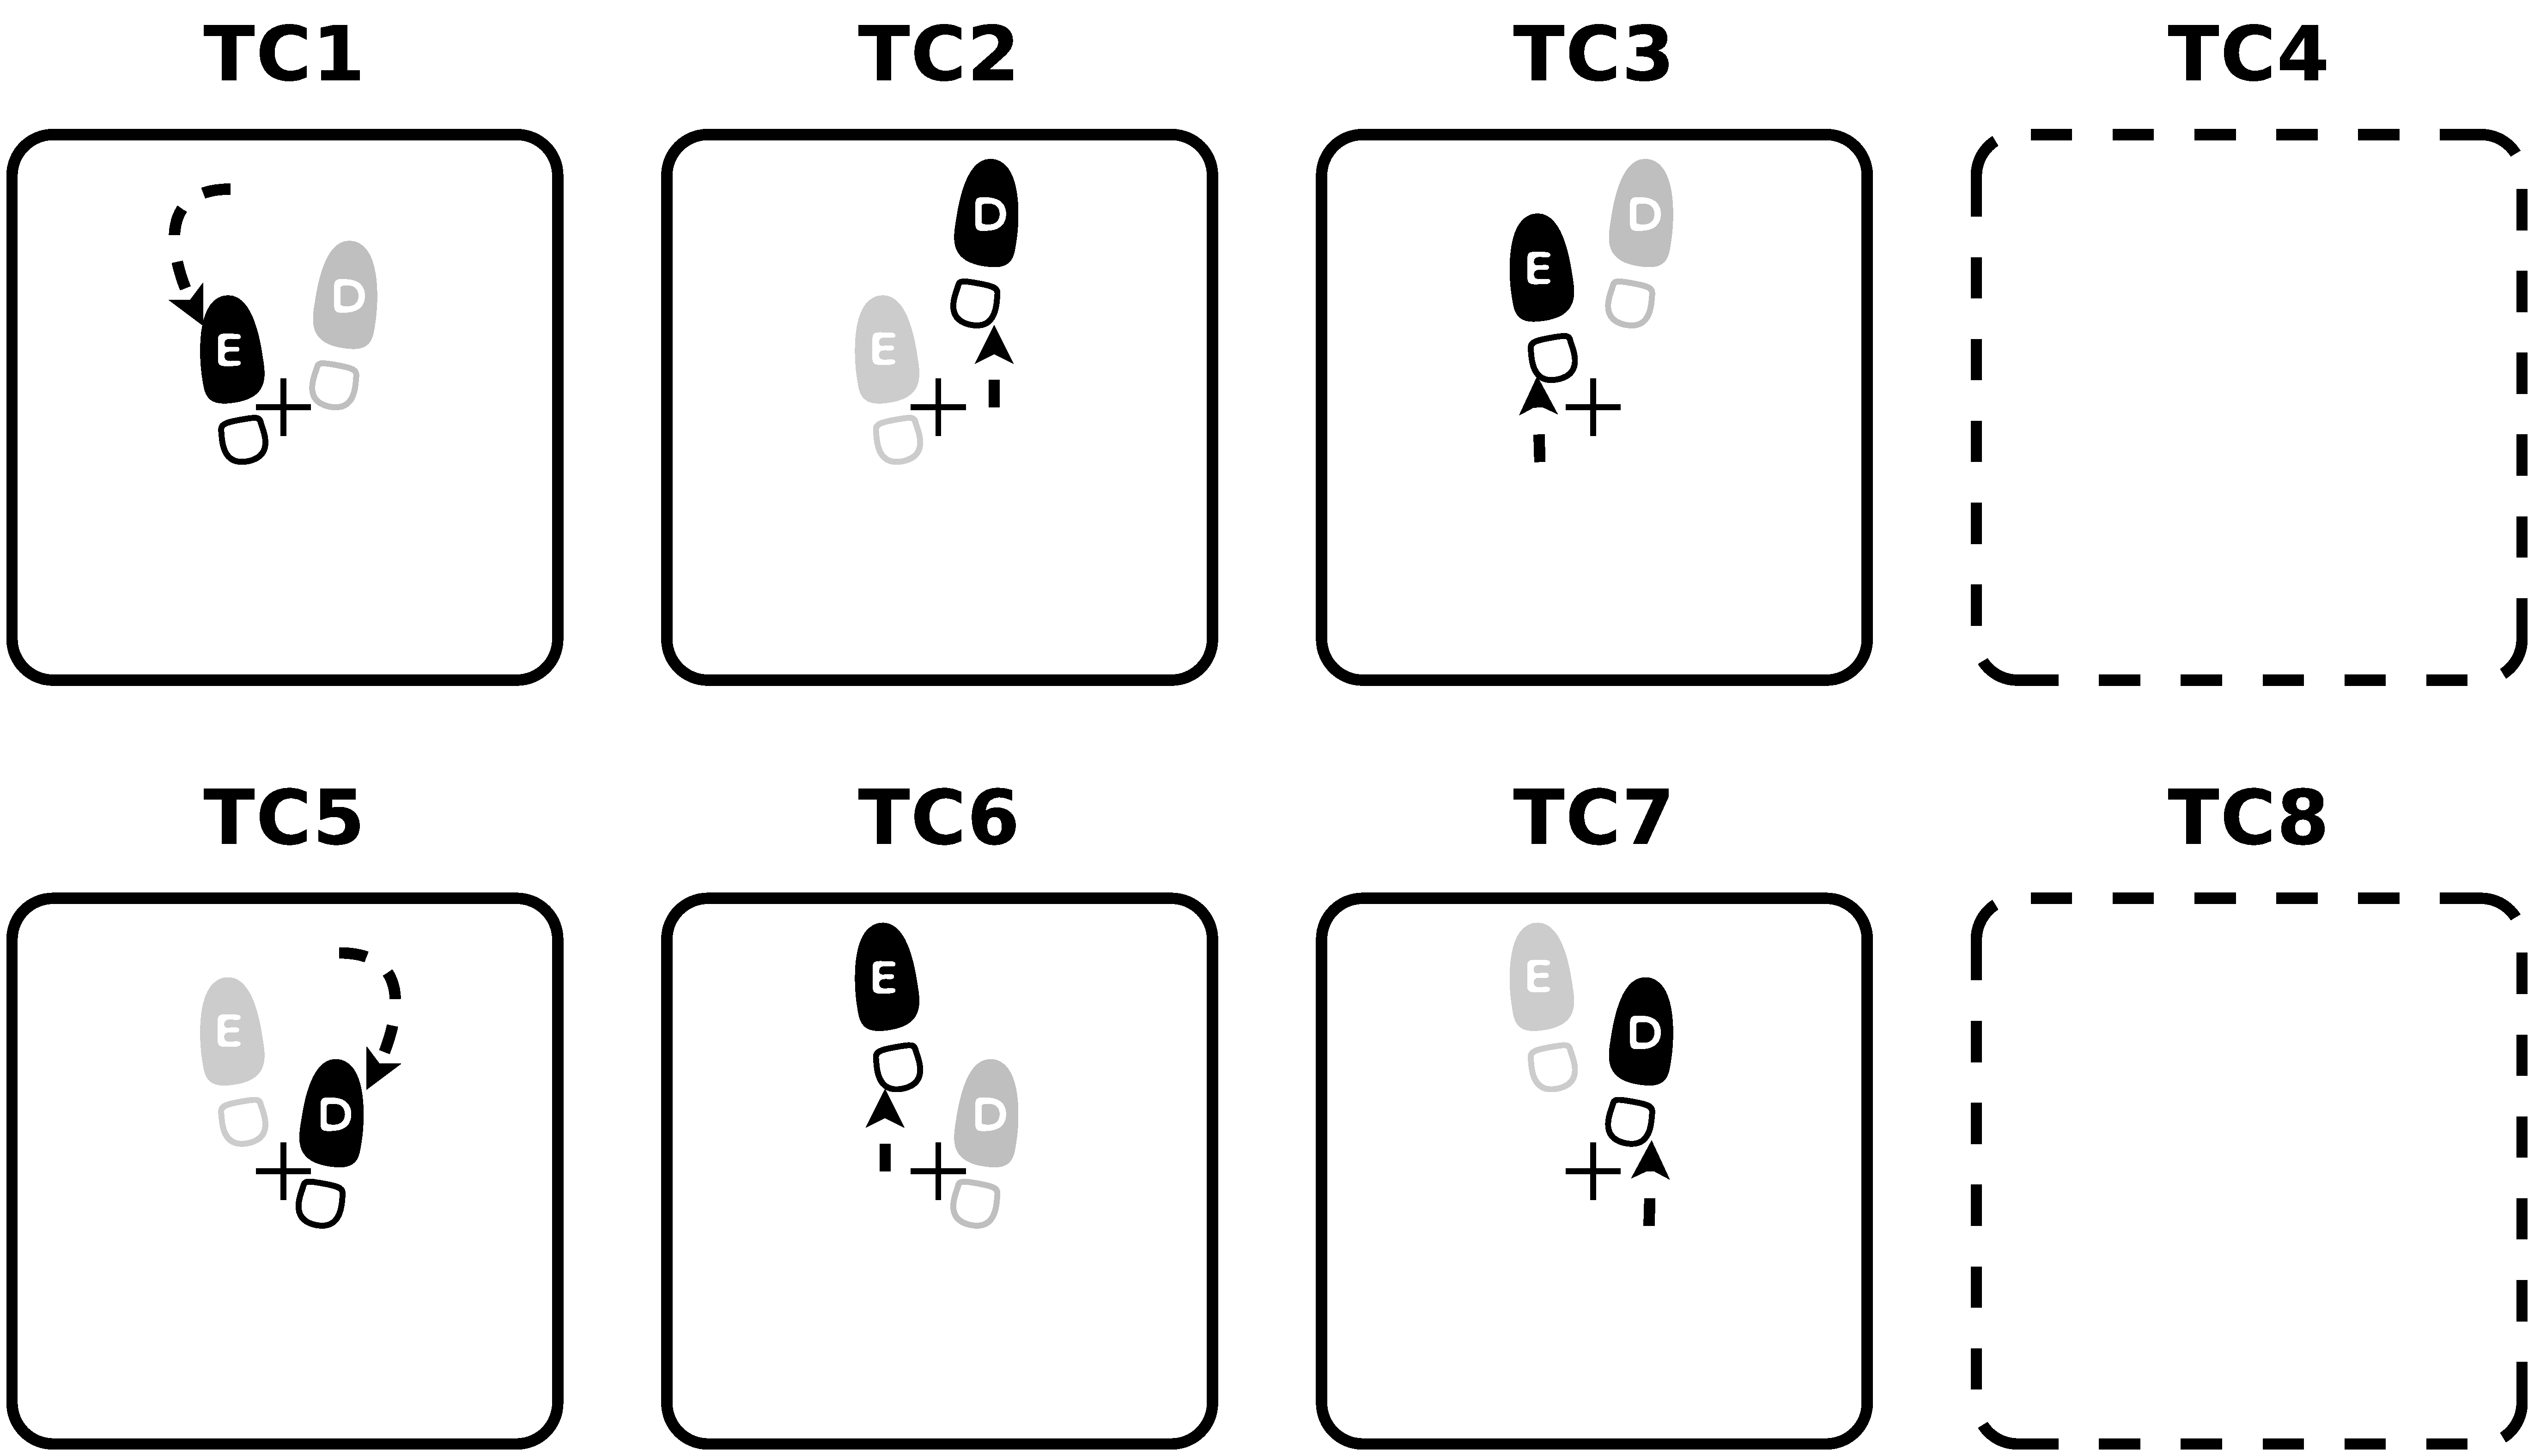
\includegraphics[width=\workboxsize]{chapters/cap-passos-footwork/samba-no-pe-b.eps}
\caption{Diagrama de tempos coreográficos para o passo de samba no pé  para atrás, $T=2~TC$.}
\label{fig:pessoa-samba-no-pe-b}
\end{figure}


A Figura \ref{fig:abc-pessoalsambape2} mostra o diagrama de tempos coreográficos para realizar a variante do passo de samba no pé,
pra atrás, explicada na Figura \ref{fig:pessoa-samba-no-pe-b}.
\begin{figure}[!h]
  \centering
\begin{abc}[name=abc-pessoalsambape2,width=0.7\linewidth]
X: 1 % start of header
K: C stafflines=1 % scale: C major
M: 2/4 %meter - compasso
%Q:1/4=80
V:1 clef=perc stem=up name="Ritmo" sname="Ritmo"
V:2 clef=perc stem=up name="TC"    sname="TC"
[V:1] |: B2  B1  B1 | B2  B1  B1 :| 
w:       ~  tchic tchic tum tchic tchic 
w: tum ~ ~ ~ ~ ~ 
w: ~ ~ ~ ~ ~ ~ 
[V:2] |: B2  B1  B1 | B2  B1  B1 :| 
w:       ~   TC1 TC2  TC3 TC5 TC6 
w:       TC7  
\end{abc}
\caption{Diagrama de tempos para a execução do passo do samba no pé para atrás.}
\label{fig:abc-pessoalsambape2}
\end{figure}

%%%%%%%%%%%%%%%%%%%%%%%%%%%%%%%%%%%%%%%%%%%%%%%%%%%%%%%%%%%%%%%%%%%%%%%%%%%%%%%%
\clearpage
\section{\Variante: Samba no pé (para adiante)}\index{Passo!Samba no pé para adiante}
A Figura \ref{fig:pessoa-samba-no-pe-adiante} mostra os movimentos necessários para executar uma variante do passo de samba no pé para adiante.
\begin{itemize}
\item Cada quadro de trabalho representa a posição dos pés em cada tempo coreográfico;
\item um tempo coreográfico tem uma duração igual a meio tempo musical (T).
\item O passo básico de samba no pé  pode ser executado de forma cíclica, de modo que 
a sequencia de passos pode executar-se como: TC1, TC2, ..., TC7, TC8, TC1, ..., etc.  
Quantas vesses se considere necessário.
\end{itemize}

\begin{figure}[!h]
  \centering
    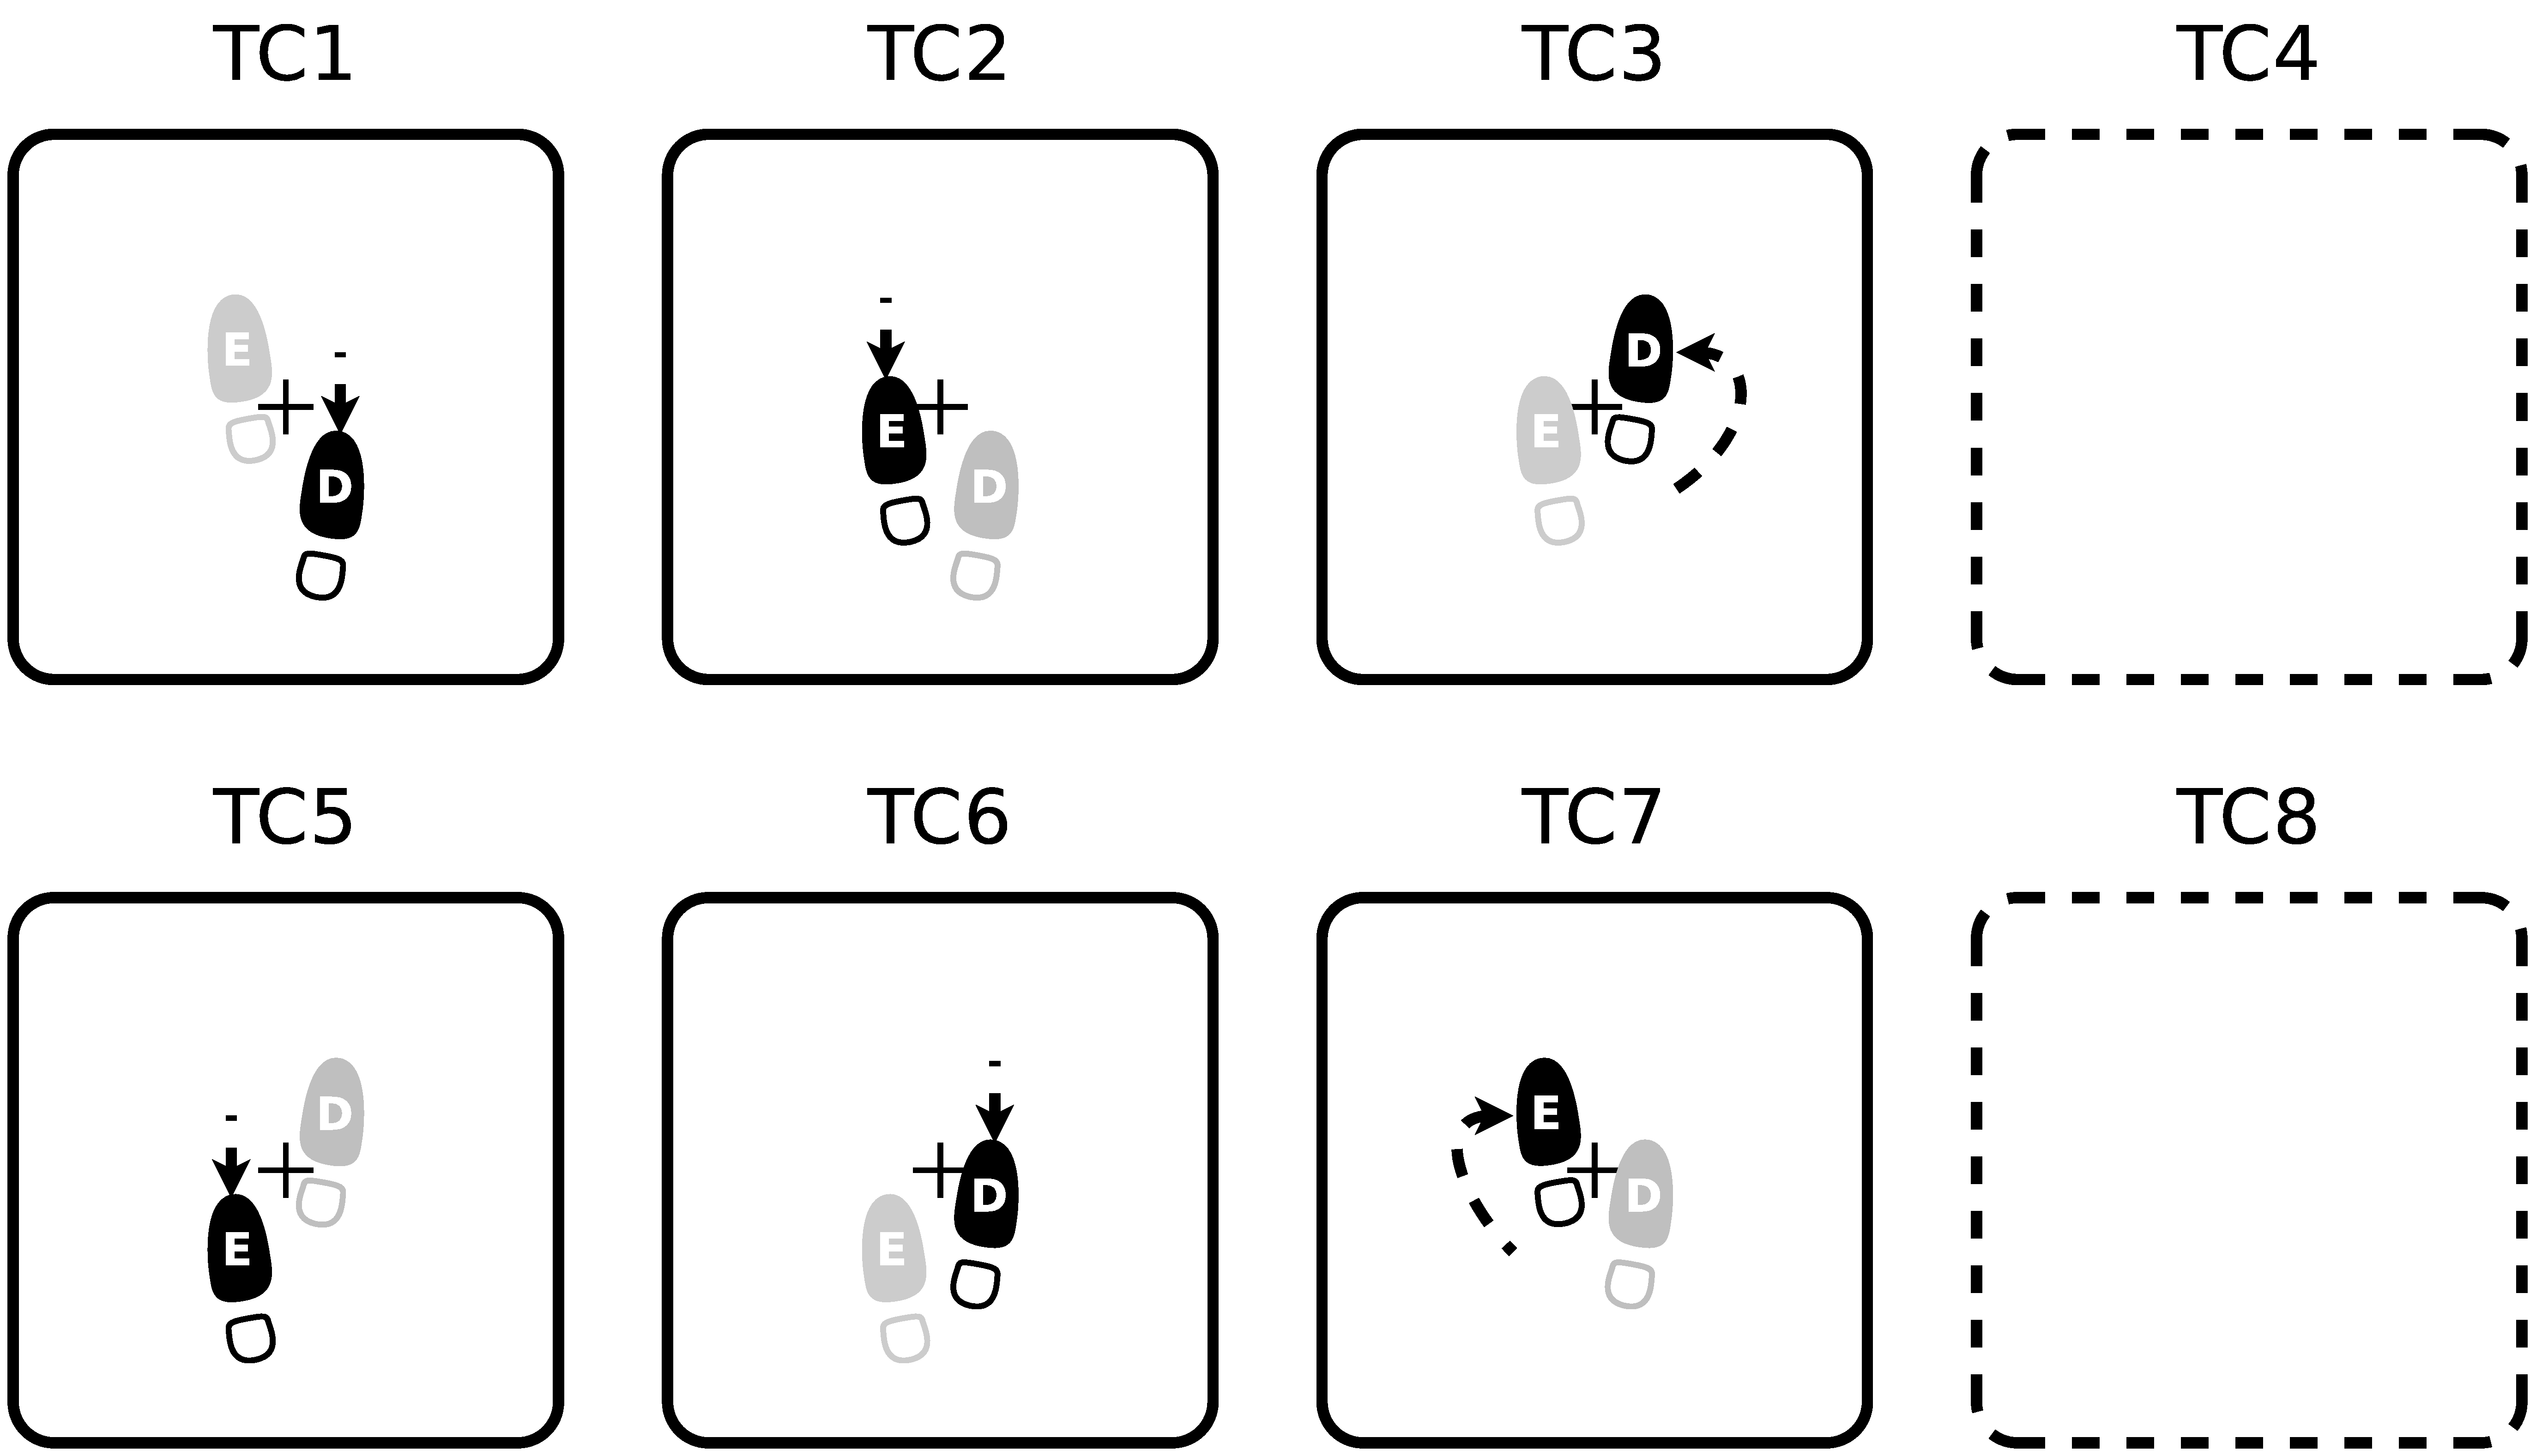
\includegraphics[width=\workboxsize]{chapters/cap-passos-footwork/samba-no-pe-adiante.eps}
\caption{Diagrama de tempos coreográficos para o passo de samba no pé para adiante, $T=2~TC$.}
\label{fig:pessoa-samba-no-pe-adiante}
\end{figure}



A Figura \ref{fig:abc-pessoalsambape-adiante1} mostra o diagrama de tempos coreográficos para realizar o passo de samba no pé,
pra adiante.
\begin{figure}[!h]
  \centering
\begin{abc}[name=abc-pessoalsambape-adiante1,width=0.7\linewidth]
X: 1 % start of header
K: C stafflines=1 % scale: C major
M: 2/4 %meter - compasso
%Q:1/4=80
V:1 clef=perc stem=up name="Ritmo" sname="Ritmo"
V:2 clef=perc stem=up name="TC"    sname="TC"
[V:1] |: B2  B1  B1 | B2  B1  B1 :| 
w:       ~  tchic tchic tum tchic tchic 
w: tum ~ ~ ~ ~ ~ 
w: ~ ~ ~ ~ ~ ~ 
[V:2] |: B2  B1  B1 | B2  B1  B1 :| 
w:       ~   TC1 TC2  TC3 TC5 TC6 
w:       TC7  
\end{abc}
\caption{Diagrama de tempos para a execução do passo do samba no pé para atrás.}
\label{fig:abc-pessoalsambape-adiante1}
\end{figure}

%%%%%%%%%%%%%%%%%%%%%%%%%%%%%%%%%%%%%%%%%%%%%%%%%%%%%%%%%%%%%%%%%%%%%%%%%%%%%%%%
\clearpage
\section{\Variante~2: Samba no pé (para adiante)}\index{Passo!Samba no pé para adiante}
A Figura \ref{fig:pessoa-samba-no-pe-adiante-b} mostra os movimentos necessários para executar uma variante do passo de samba no pé para adiante.
\begin{itemize}
\item Cada quadro de trabalho representa a posição dos pés em cada tempo coreográfico;
\item um tempo coreográfico tem uma duração igual a meio tempo musical (T).
\item O passo básico de samba no pé  pode ser executado de forma cíclica, de modo que 
a sequencia de passos pode executar-se como: TC1, TC2, ..., TC7, TC8, TC1, ..., etc.  
Quantas vesses se considere necessário.
\end{itemize}


\begin{figure}[!h]
  \centering
    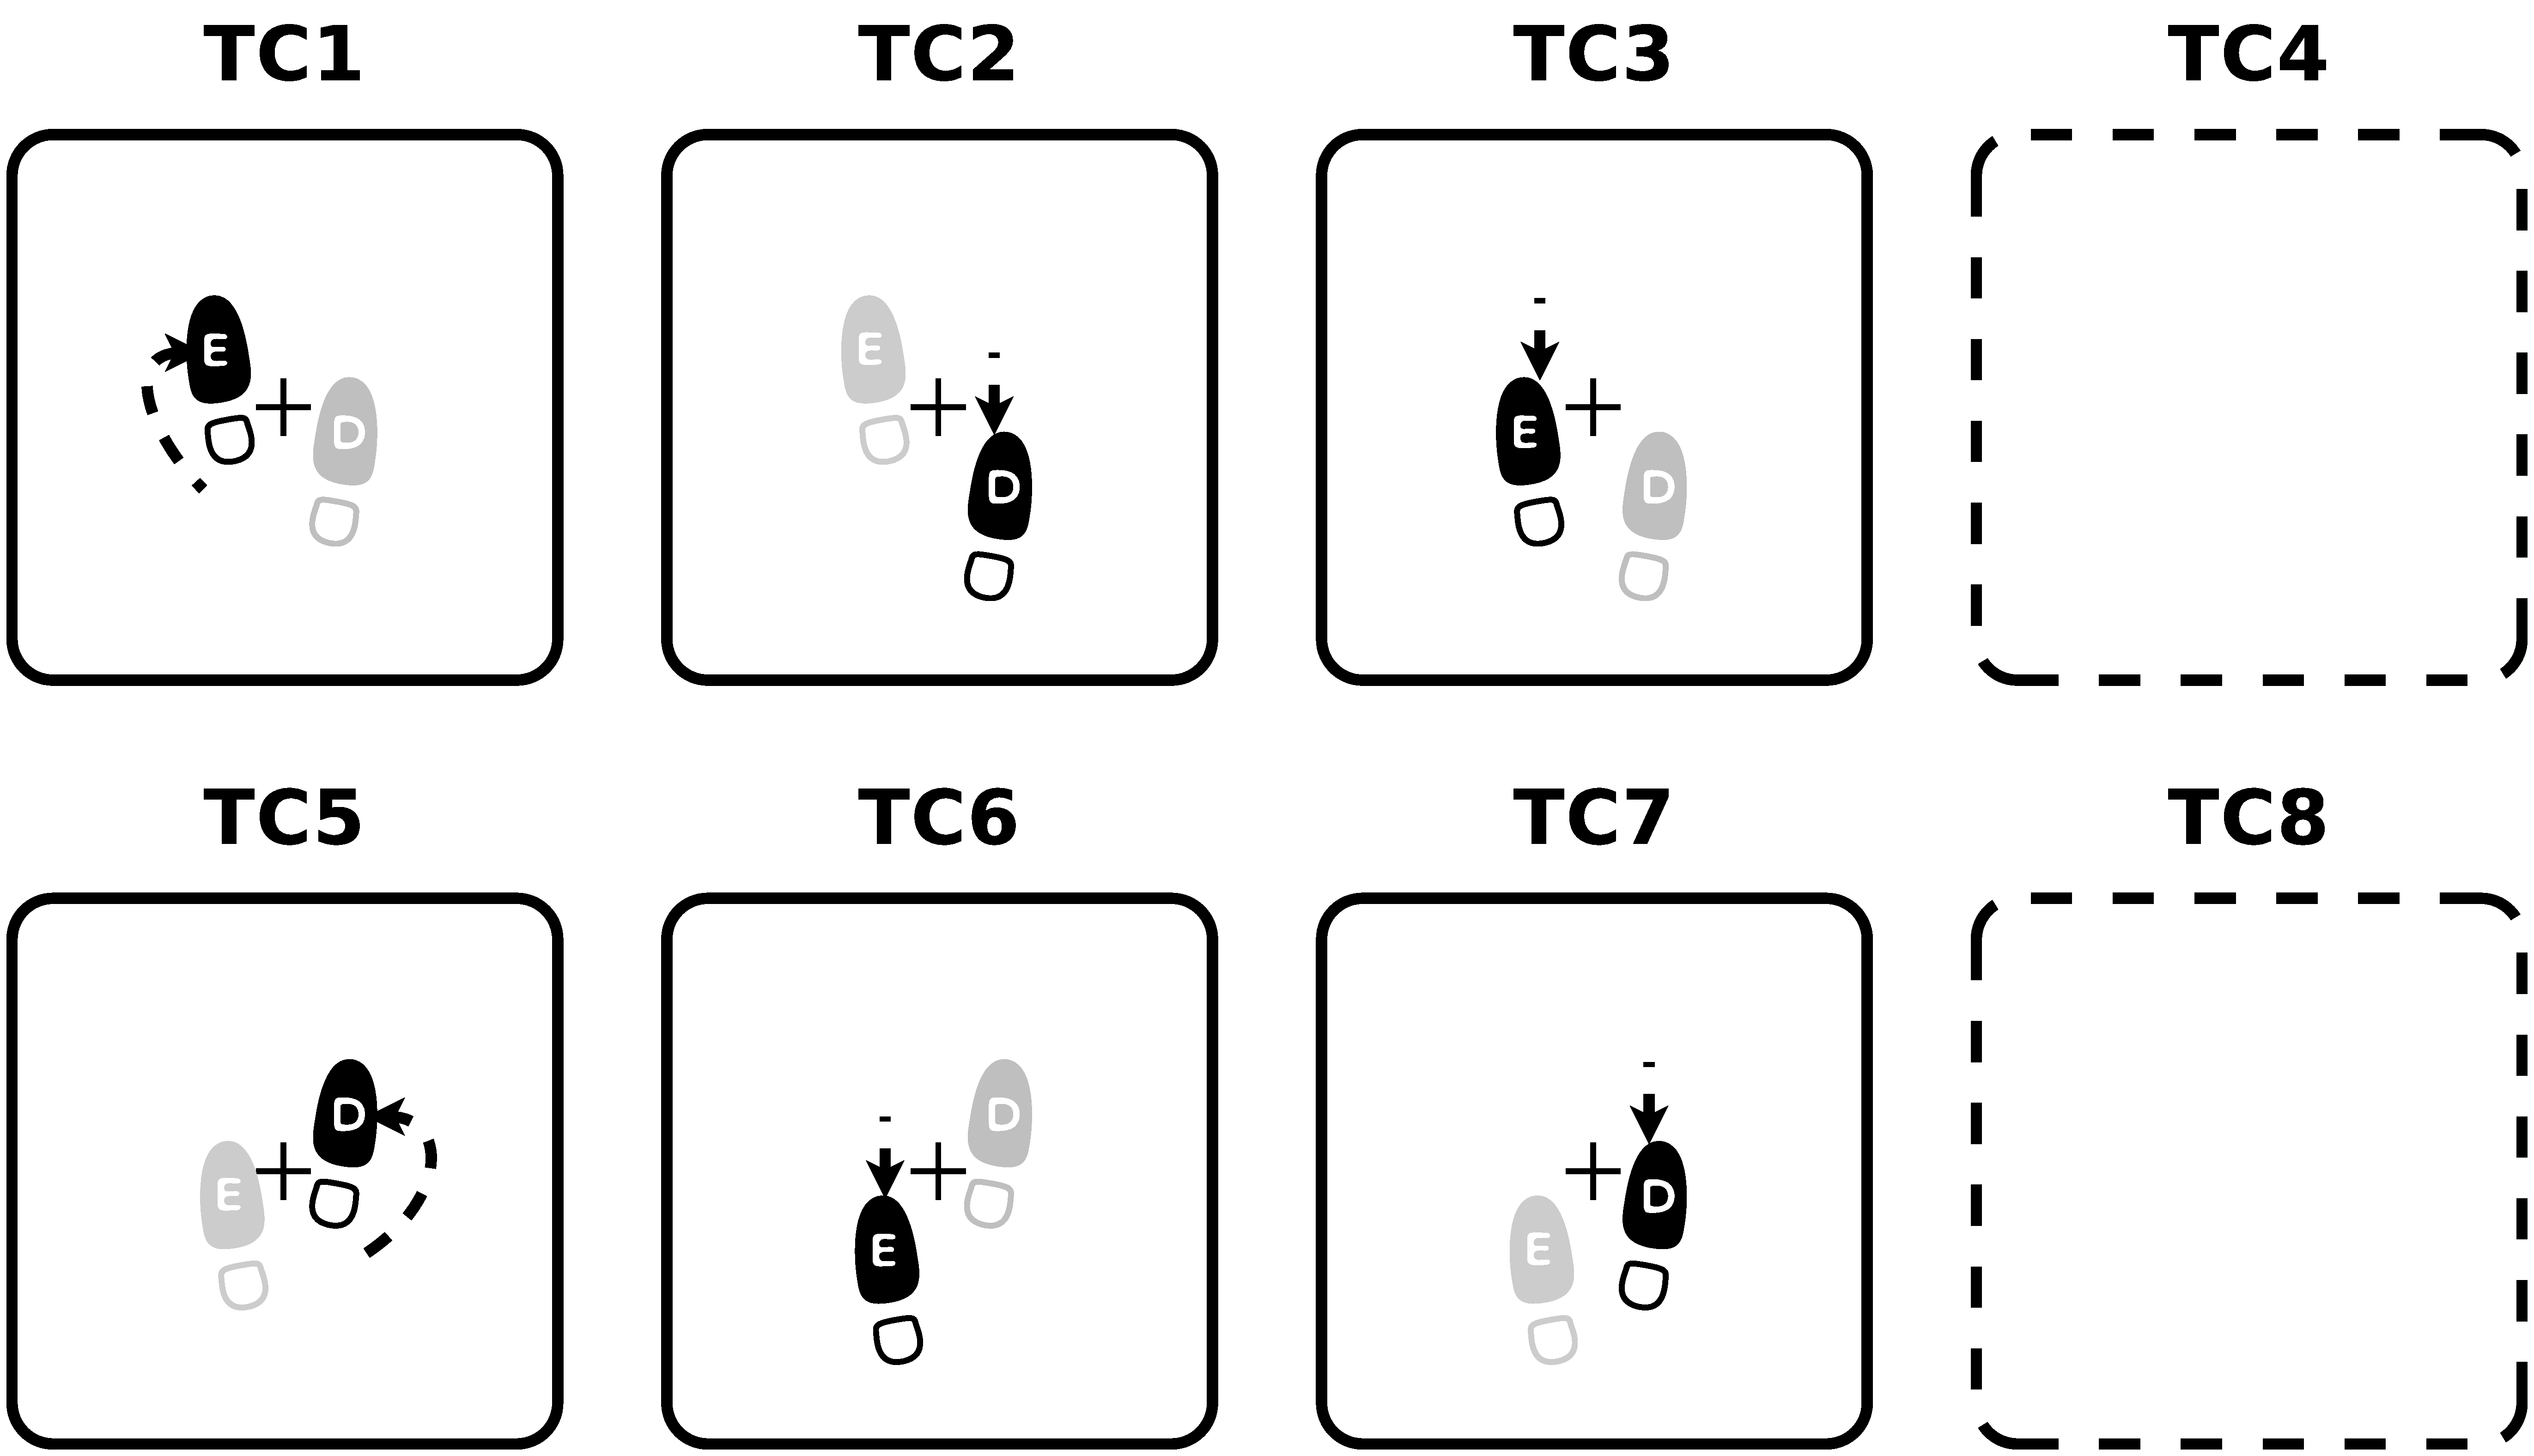
\includegraphics[width=\workboxsize]{chapters/cap-passos-footwork/samba-no-pe-adiante-b.eps}
\caption{Diagrama de tempos coreográficos para o passo de samba no pé para adiante, $T=2~TC$.}
\label{fig:pessoa-samba-no-pe-adiante-b}
\end{figure}


A Figura \ref{fig:abc-pessoalsambape-adiante2} mostra o diagrama de tempos coreográficos para realizar a variante do passo de samba no pé,
pra adiante, explicada na Figura \ref{fig:pessoa-samba-no-pe-adiante-b}.

\begin{figure}[!h]
  \centering
\begin{abc}[name=abc-pessoalsambape-adiante2,width=0.7\linewidth]
X: 1 % start of header
K: C stafflines=1 % scale: C major
M: 2/4 %meter - compasso
%Q:1/4=80
V:1 clef=perc stem=up name="Ritmo" sname="Ritmo"
V:2 clef=perc stem=up name="TC"    sname="TC"
[V:1] |: B2  B1  B1 | B2  B1  B1 :| 
w:       ~  tchic tchic tum tchic tchic 
w: tum ~ ~ ~ ~ ~ 
w: ~ ~ ~ ~ ~ ~ 
[V:2] |: B2  B1  B1 | B2  B1  B1 :| 
w:       ~   TC1 TC2  TC3 TC5 TC6 
w:       TC7  
\end{abc}
\caption{Diagrama de tempos para a execução do passo do samba no pé para adiante.}
\label{fig:abc-pessoalsambape-adiante2}
\end{figure}

%%%%%%%%%%%%%%%%%%%%%%%%%%%%%%%%%%%%%%%%%%%%%%%%%%%%%%%%%%%%%%%%%%%%%%%%%%%%%%%%
% da tesoura dupla
\clearpage
\section{ \Variante: Tesoura }\index{Passo!Tesoura}


A Figura \ref{fig:pessoa-tesoura} mostra os movimentos necessários para executar uma variante do passo chamado tesoura.
\begin{itemize}
\item Cada quadro de trabalho representa a posição dos pés em cada tempo coreográfico;
\item um tempo coreográfico tem uma duração igual a meio tempo musical (T).
\item O passo básico de samba no pé  pode ser executado de forma cíclica, de modo que 
a sequencia de passos pode executar-se como: TC1, TC2, TC1, TC2, ..., etc.  
Quantas vesses se considere necessário.
\end{itemize}

\begin{figure}[!h]
  \centering
    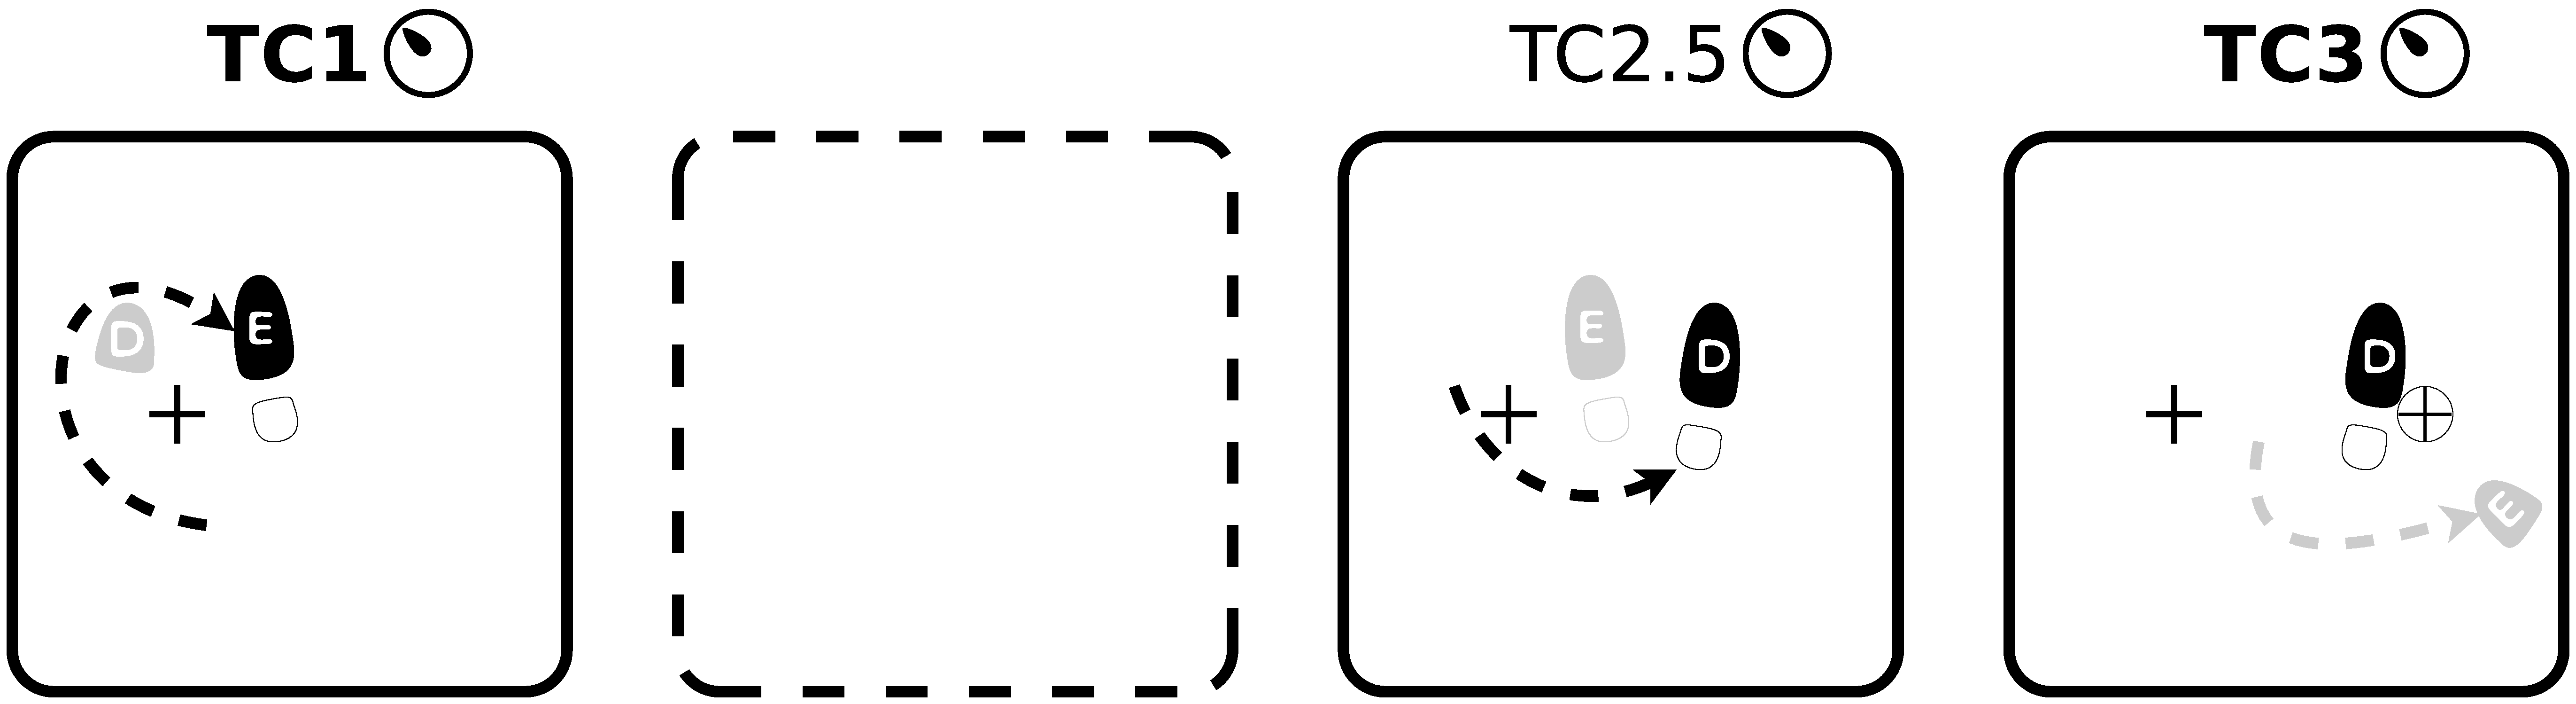
\includegraphics[width=\workboxsize]{chapters/cap-passos-footwork/tesoura.eps}
\caption{Diagrama de tempos coreográficos para o passo tesoura, $T=2~TC$.}
\label{fig:pessoa-tesoura}
\end{figure}




A Figura \ref{fig:abc-pessoaltesoura} mostra o diagrama de tempos coreográficos para realizar a variante do passo de samba no pé,
pra adiante, explicada na Figura \ref{fig:pessoa-tesoura}.

\begin{figure}[!h]
  \centering
\begin{abc}[name=abc-pessoaltesoura,width=0.7\linewidth]
X: 1 % start of header
K: C stafflines=1 % scale: C major
M: 2/4 %meter - compasso
%Q:1/4=80
V:1 clef=perc stem=up name="Ritmo" sname="Ritmo"
V:2 clef=perc stem=up name="TC"    sname="TC"
[V:1] |: B2 B1    B1    | B2  B1    B1  :| 
w:       ~  tchic tchic   ~   tchic tchic
w:       tum ~    ~       tum ~ ~ 
w: ~ ~ ~ ~ ~ ~ 
[V:2] |: B2  B3/2  B1/2  | B2  B3/2  B1/2  :| 
w:       ~   TC1   TC2.5   ~   TC1   TC2.5 
w:       TC3 ~     ~       TC3  
\end{abc}
\caption{Diagrama de tempos para a execução do passo tesoura.}
\label{fig:abc-pessoaltesoura}
\end{figure}

%%%%%%%%%%%%%%%%%%%%%%%%%%%%%%%%%%%%%%%%%%%%%%%%%%%%%%%%%%%%%%%%%%%%%%%%%%%%%%%%
\clearpage
\section{\Variante: Balança corre corre}\index{Passo!Balança corre corre}


A Figura \ref{fig:pessoa-balanca-corre-corre} mostra os movimentos necessários para executar uma variante do passo chamado balança corre corre.
\begin{itemize}
\item Cada quadro de trabalho representa a posição dos pés em cada tempo coreográfico;
\item um tempo coreográfico tem uma duração igual a meio tempo musical (T).
\item O passo básico de samba no pé  pode ser executado de forma cíclica, de modo que 
a sequencia de passos pode executar-se como: TC1, TC2, ..., TC5, TC6, TC1, TC2, ..., etc.  
Quantas vesses se considere necessário.
\end{itemize}

\begin{figure}[!h]
  \centering
    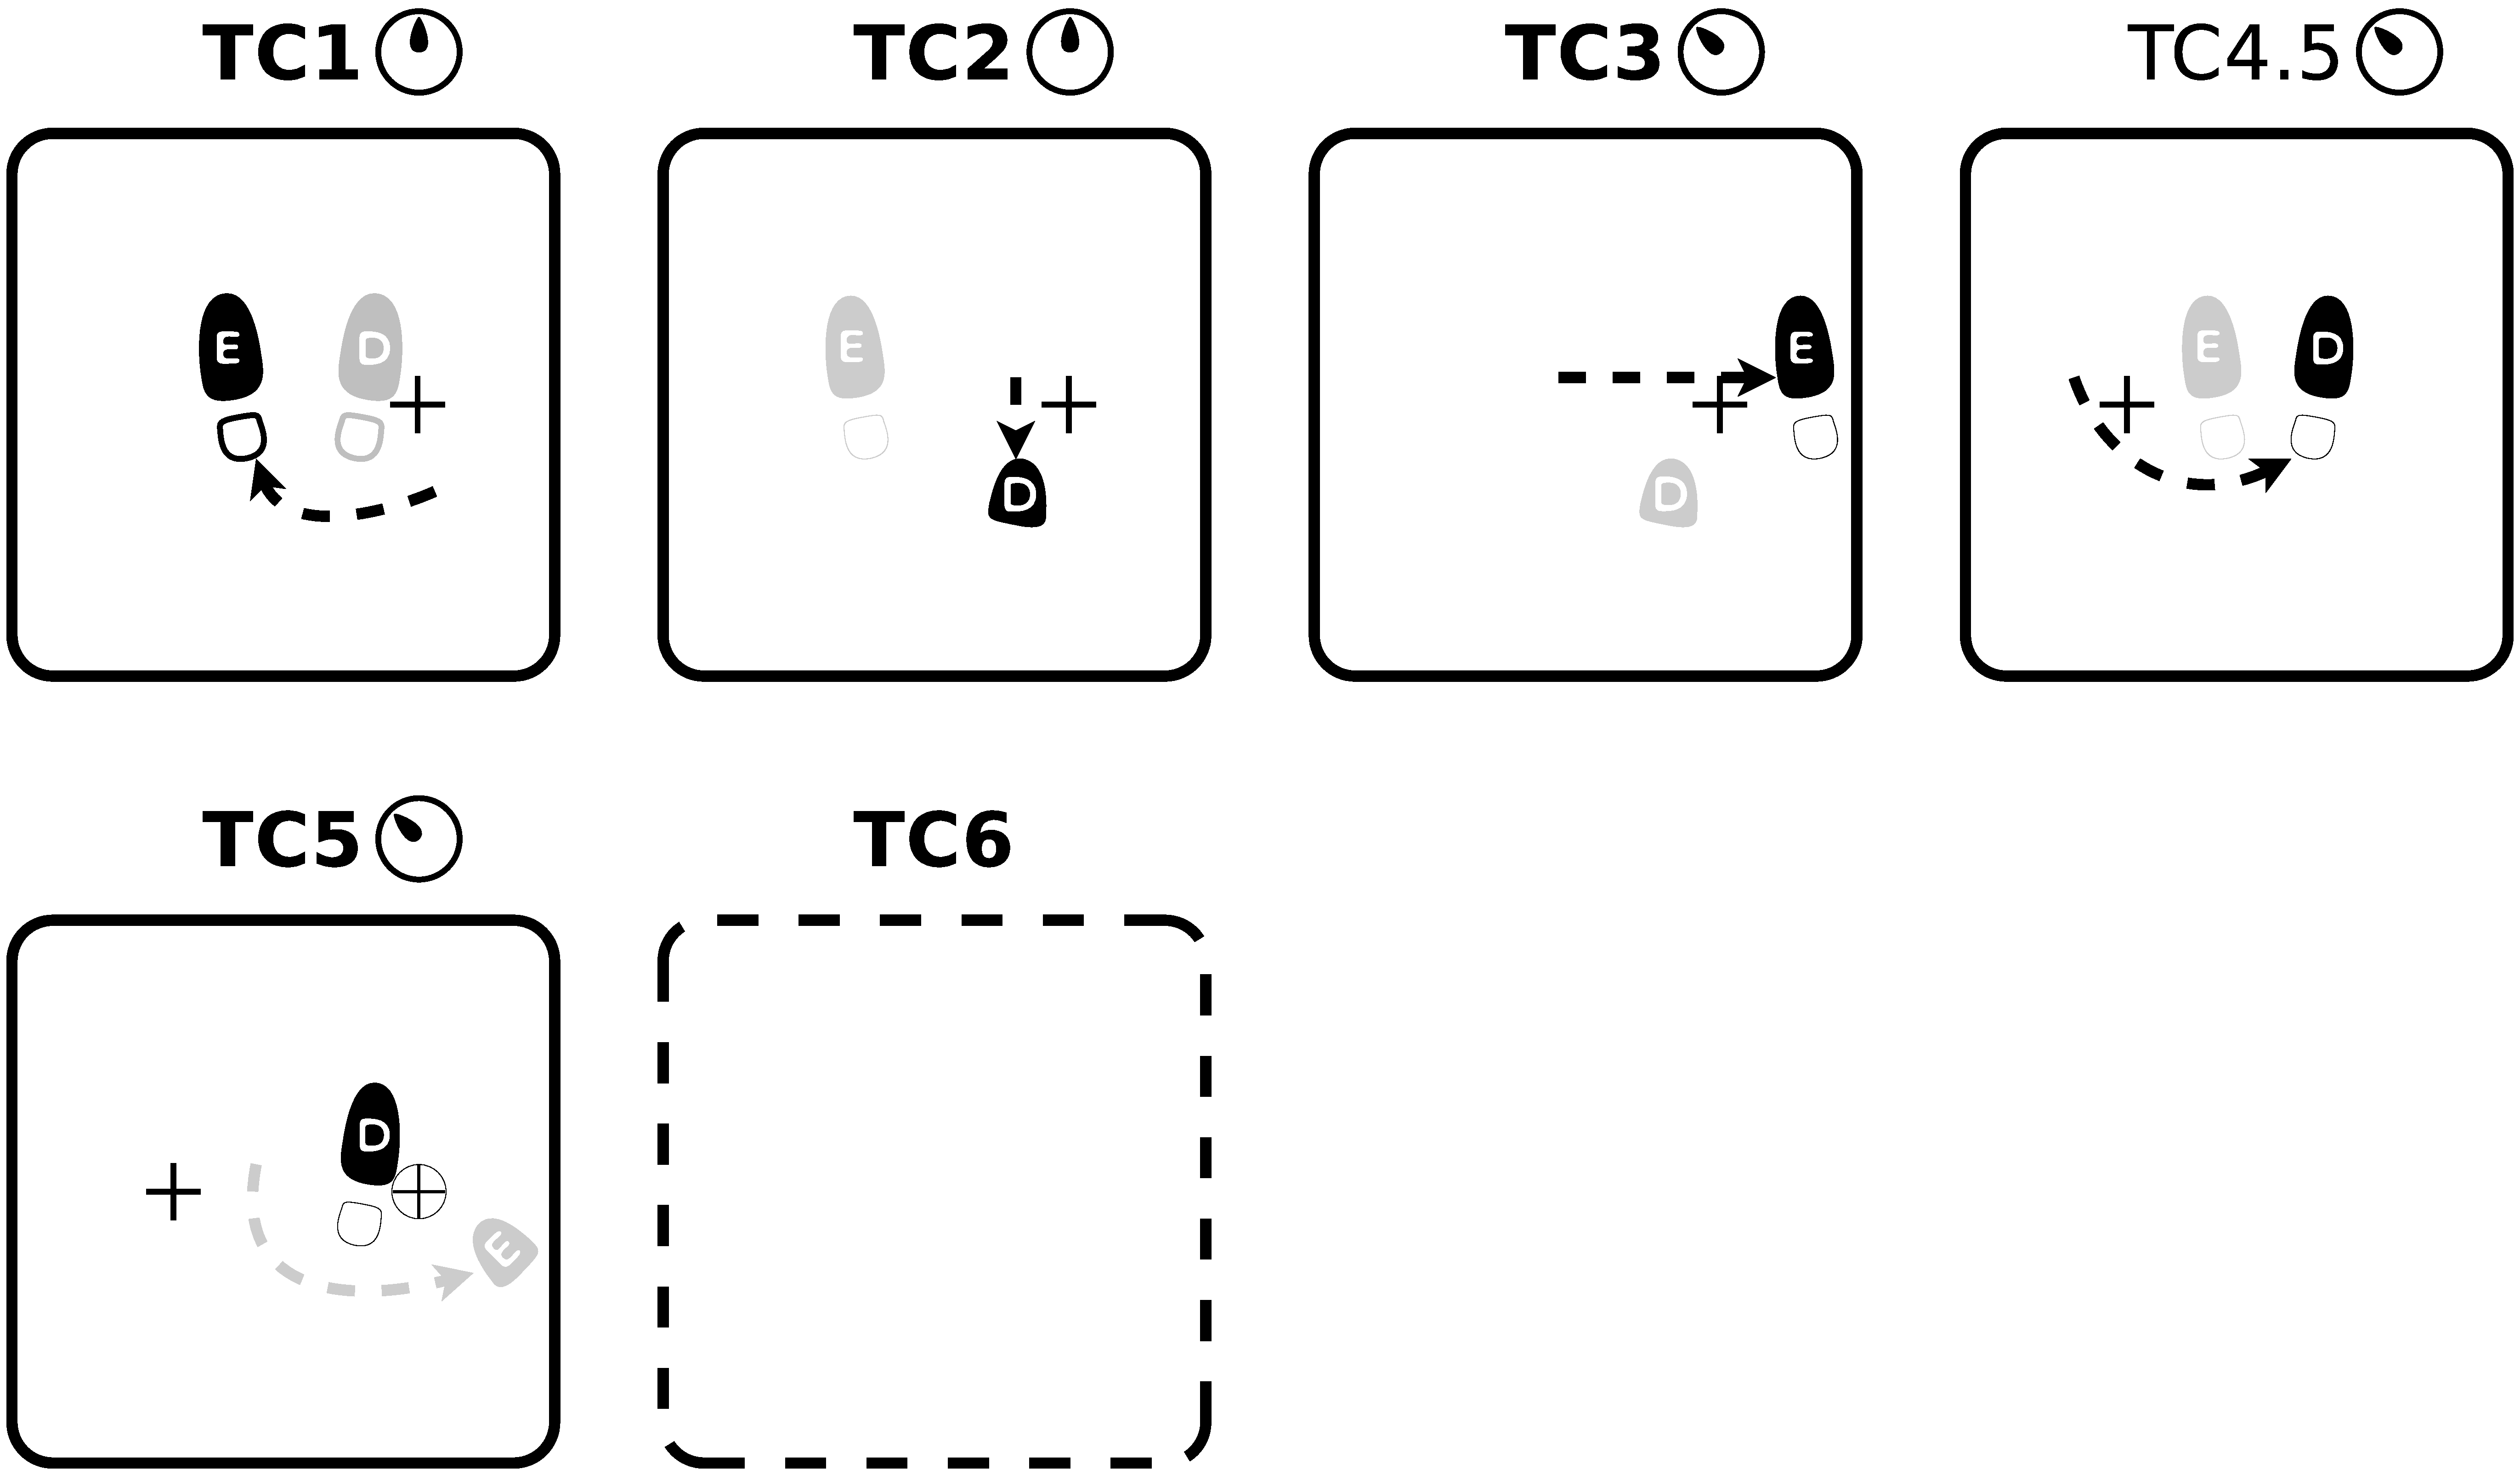
\includegraphics[width=\workboxsize]{chapters/cap-passos-footwork/balanca-corre-corre.eps}
\caption{Diagrama de tempos coreográficos para o passo balança corre corre, $T=2~TC$.}
\label{fig:pessoa-balanca-corre-corre}
\end{figure}




A Figura \ref{fig:abc-pessoal-balanca-corre-corre} mostra o diagrama de tempos coreográficos para realizar a variante do passo balanca corre corre,
explicada na Figura \ref{fig:pessoa-balanca-corre-corre}.

\begin{figure}[!h]
  \centering
\begin{abc}[name=abc-pessoal-balanca-corre-corre,width=1.0\linewidth]
X: 1 % start of header
K: C stafflines=1 % scale: C major
M: 2/4 %meter - compasso
%Q:1/4=80
V:1 clef=perc stem=up name="Ritmo" sname="Ritmo"
V:2 clef=perc stem=up name="TC"    sname="TC"
[V:1] |: B2 B1    B1    | B2  B1    B1   | B2  B1    B1 :| 
w:       ~  tchic tchic   tum tchic tchic  ~   ~     ~
w:       tum ~    ~       ~   ~     ~      tum tchic tchic
w: ~ ~ ~ ~ ~ ~ 
[V:2] |: B2  B1  B1   | B3/2 B1/2  B2    | B1  B1  B3/2 B1/2   :| 
w:       ~   TC1 TC2    TC3  TC4.5 TC5     ~   ~   ~    ~  
w:       TC5 ~   ~      ~    ~     ~       TC1 TC2 TC3  TC4.5
\end{abc}
\caption{Diagrama de tempos para a execução do passo balança corre corre.}
\label{fig:abc-pessoal-balanca-corre-corre}
\end{figure}

%%%%%%%%%%%%%%%%%%%%%%%%%%%%%%%%%%%%%%%%%%%%%%%%%%%%%%%%%%%%%%%%%%%%%%%%%%%%%%%%
\clearpage
\section{ \Variante: Pica-pau }\index{Passo!Pica-pau}

A Figura \ref{fig:pessoa-pica-pau} mostra os movimentos necessários para executar uma variante do passo chamado pica-pau.
\begin{itemize}
\item Cada quadro de trabalho representa a posição dos pés em cada tempo coreográfico;
\item um tempo coreográfico tem uma duração igual a meio tempo musical (T).
\item O passo básico de samba no pé  pode ser executado de forma cíclica, de modo que 
a sequencia de passos pode executar-se como: TC1, TC2, ..., TC7, TC8, TC1, TC2, ..., etc.  
Quantas vesses se considere necessário.
\end{itemize}

\begin{figure}[!h]
  \centering
    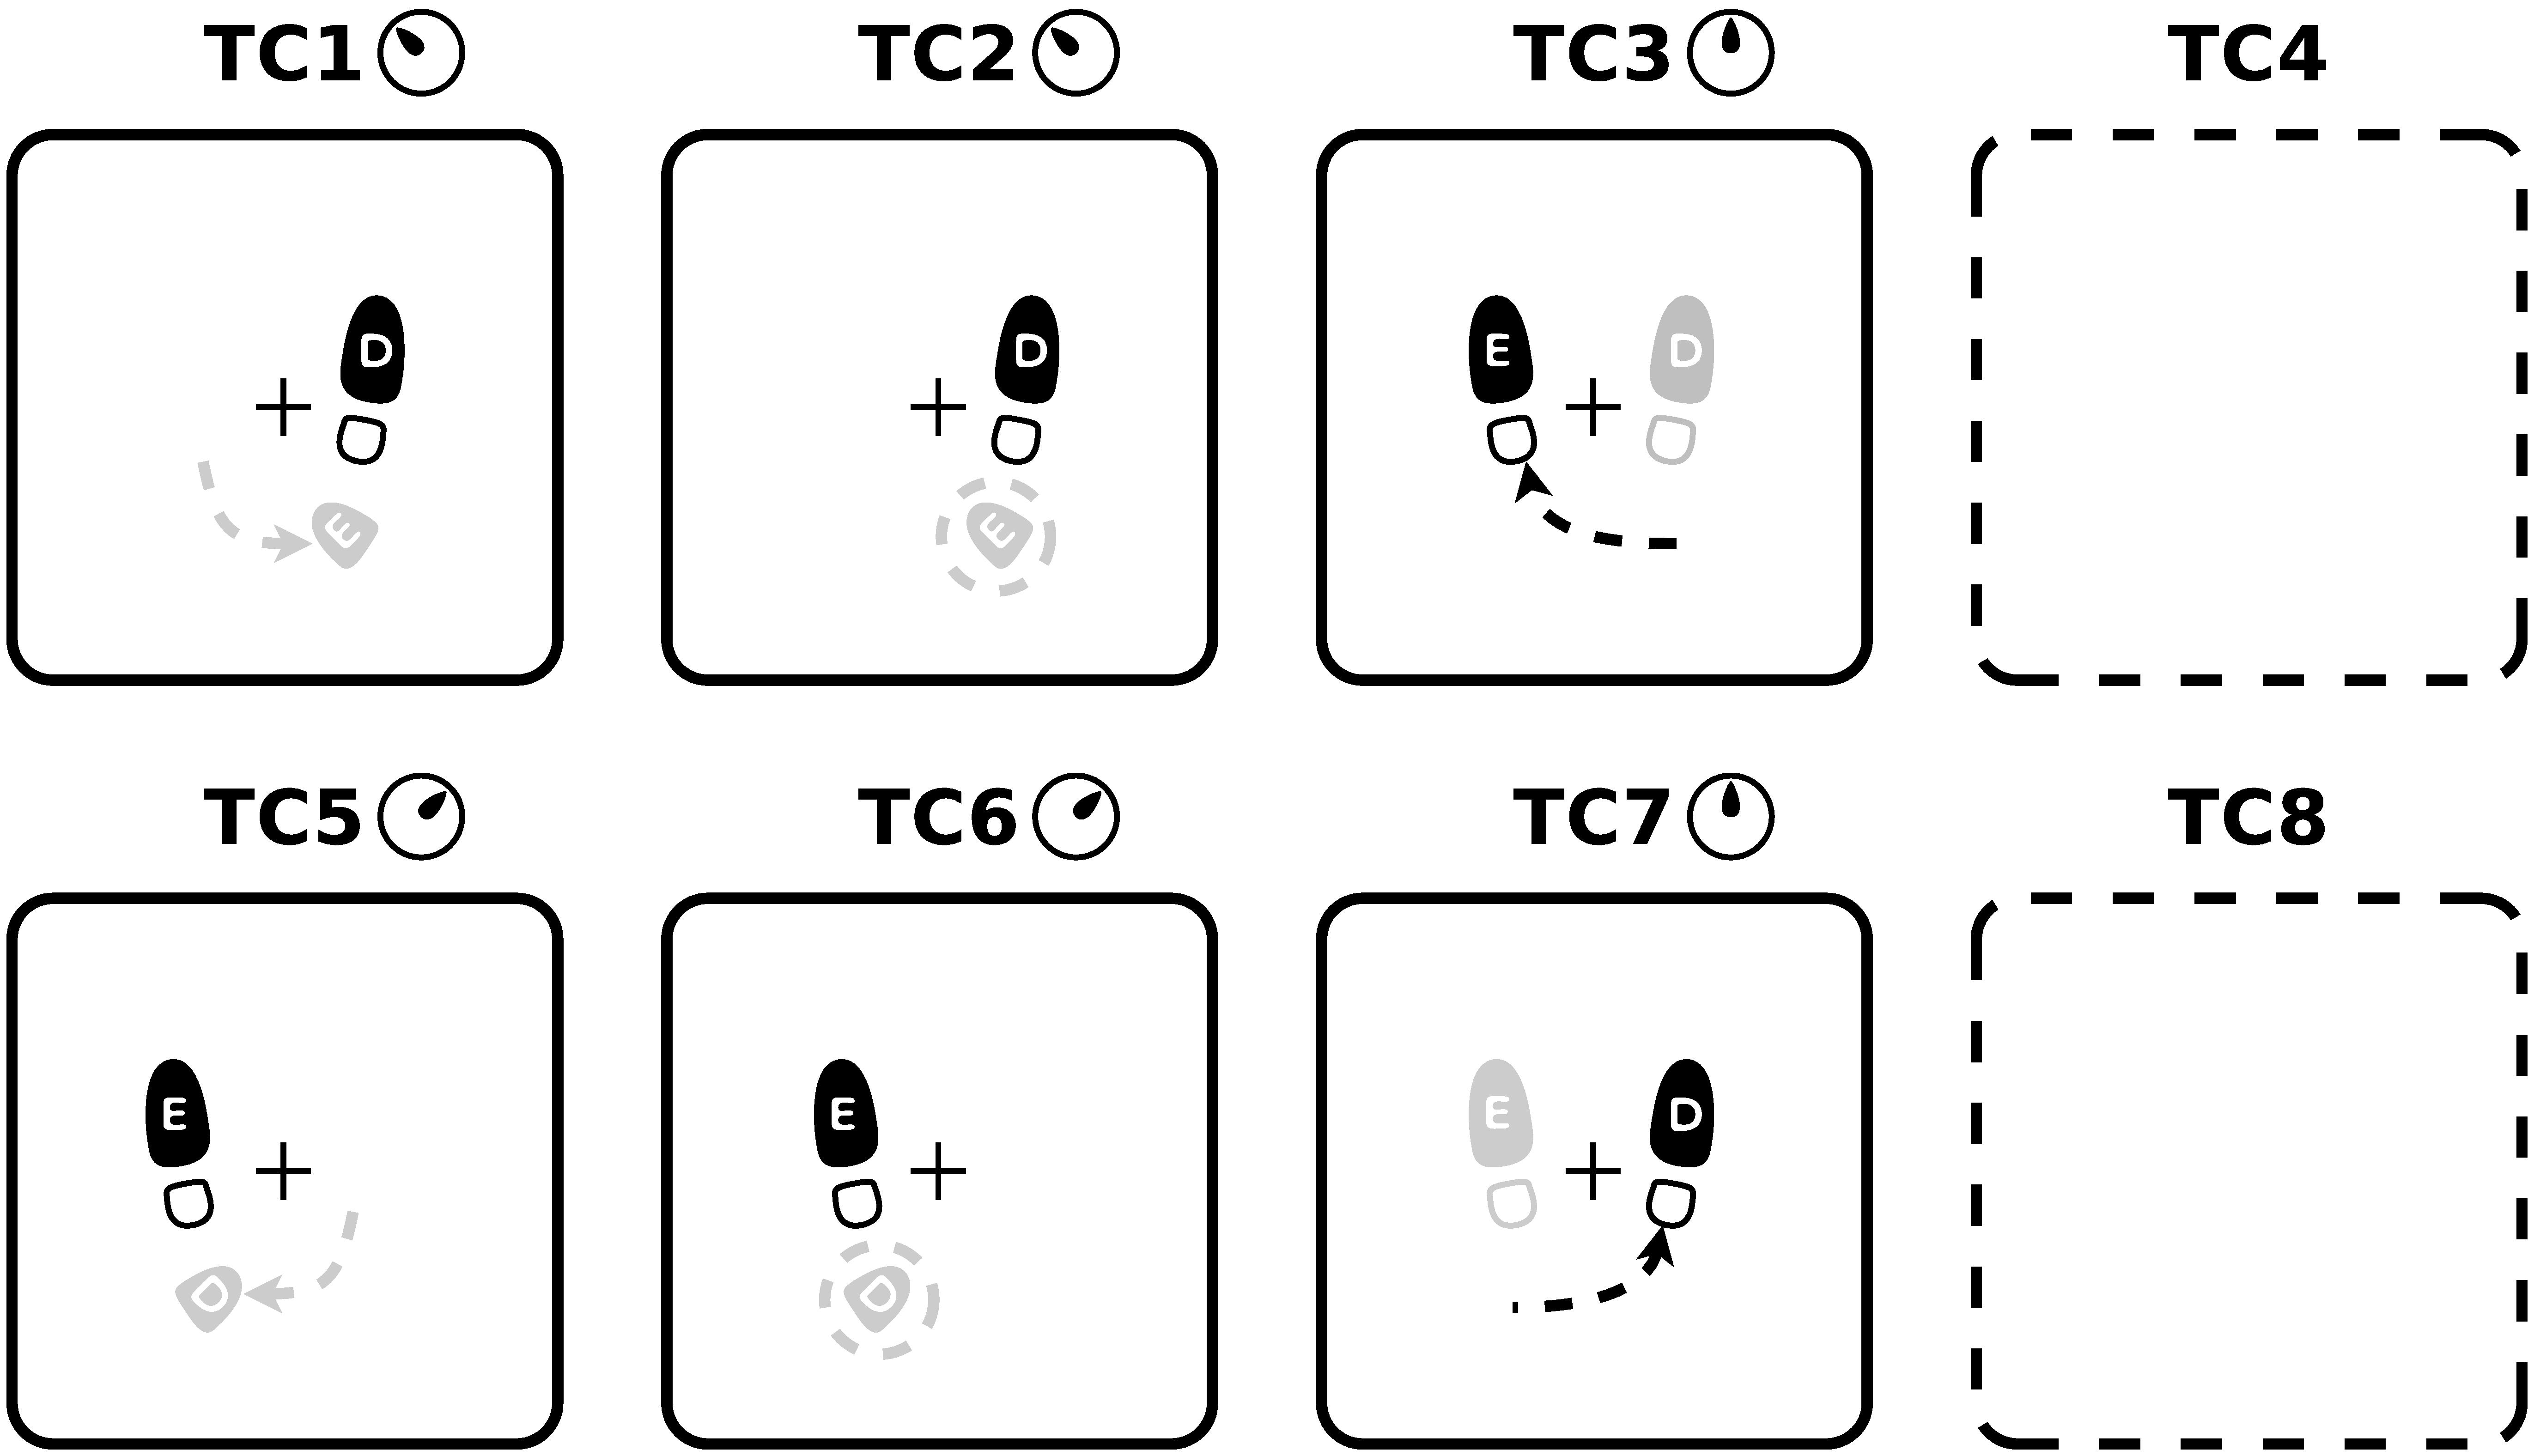
\includegraphics[width=\workboxsize]{chapters/cap-passos-footwork/pica-pau.eps}
\caption{Diagrama de tempos coreográficos para o passo pica-pau, $T=2~TC$.}
\label{fig:pessoa-pica-pau}
\end{figure}




A Figura \ref{fig:abc-pessoal-pica-pau} mostra o diagrama de tempos coreográficos para realizar o passo pica-pau,
explicada na Figura \ref{fig:pessoa-pica-pau}.

\begin{figure}[!h]
  \centering
\begin{abc}[name=abc-pessoal-pica-pau,width=0.7\linewidth]
X: 1 % start of header
K: C stafflines=1 % scale: C major
M: 2/4 %meter - compasso
%Q:1/4=80
V:1 clef=perc stem=up name="Ritmo" sname="Ritmo"
V:2 clef=perc stem=up name="TC"    sname="TC"
[V:1] |: B2  B1  B1 | B2  B1  B1 :| 
w:       ~  tchic tchic tum tchic tchic 
w: tum ~ ~ ~ ~ ~ 
w: ~ ~ ~ ~ ~ ~ 
[V:2] |: B2  B1  B1 | B2  B1  B1 :| 
w:       ~   TC1 TC2  TC3 TC5 TC6 
w:       TC7  
\end{abc}
\caption{Diagrama de tempos para a execução do passo pica-pau.}
\label{fig:abc-pessoal-pica-pau}
\end{figure}



%%%%%%%%%%%%%%%%%%%%%%%%%%%%%%%%%%%%%%%%%%%%%%%%%%%%%%%%%%%%%%%%%%%%%%%%%%%%%%%%
\clearpage
\section{\Variante: Escovinha (para adiante)}\index{Passo!Escovinha para adiante}

A Figura \ref{fig:abc-pessoalescovinha2} mostra o diagrama de tempos coreográficos para realizar o passo escovinha,
para adiante, os movimentos nos tempos coreográficos serão explicados na Figura \ref{fig:pessoalescovinha2}.

\begin{figure}[!h]
  \centering
\begin{abc}[name=abc-pessoalescovinha2,width=1.0\linewidth]
X: 1 % start of header
K: C stafflines=1 % scale: C major
M: 2/4 %meter - compasso
%Q:1/4=80
V:1 clef=perc stem=up name="Ritmo" sname="Ritmo"
V:2 clef=perc stem=up name="TC"    sname="TC"
[V:1] |: B2  B1  B1 | B2  B1  B1 :| 
w:       ~  tchic tchic tum tchic tchic 
w: tum ~ ~ ~ ~ ~ 
w: ~ ~ ~ ~ ~ ~ 
[V:2] |: B3/2 B1/2 B1/2  B1/2  B1/2 B1/2 | B3/2 B1/2  B1/2 B1/2  B1/2 B1/2 :| 
w:       ~   ~     TC1   TC1.5 TC2  TC2.5  TC3  TC4.5 TC5  TC5.5 TC6  TC6.5 
w:       TC7 TC8.5
\end{abc}
\caption{Diagrama de tempos para a execução do passo escovinha para adiante.}
\label{fig:abc-pessoalescovinha2}
\end{figure}


A Figura \ref{fig:pessoalescovinha2} mostra o diagrama de tempos coreográficos para realizar o passo escovinha, para adiante.
\begin{itemize}
\item Cada quadro de trabalho representa a posição dos pés em cada tempo coreográfico;
\item um tempo coreográfico tem uma duração igual a meio tempo musical (T).
\item O passo básico de samba no pé  pode ser executado de forma cíclica, de modo que 
a sequencia de passos pode executar-se como: TC1, TC2, ..., TC7, TC8, TC1, ..., etc.  
Quantas vesses se considere necessário.
\end{itemize}


\begin{sidewaysfigure}[h]
  \centering
    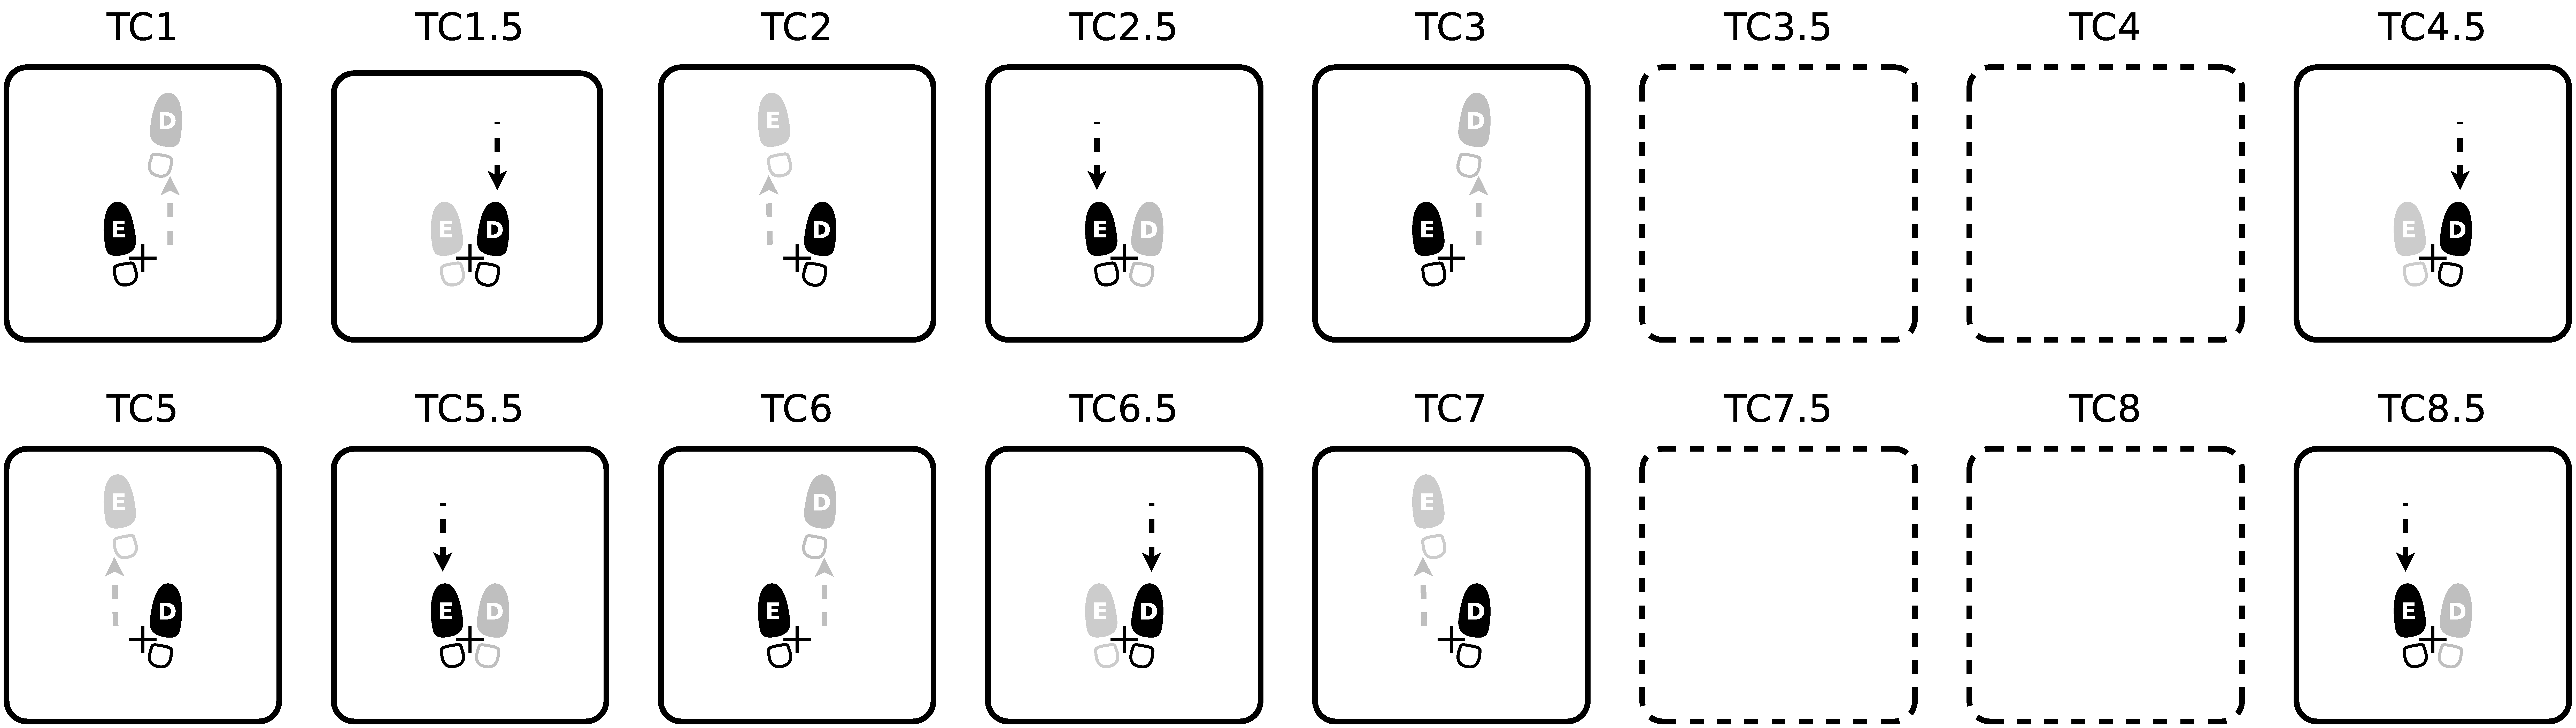
\includegraphics[width=\textwidth]{chapters/cap-passos-footwork/escovinha2.eps}
\caption{Diagrama detalhado de tempos coreográficos para a escovinha, $T=2~TC$.}
\label{fig:pessoalescovinha2}
\end{sidewaysfigure}


%%%%%%%%%%%%%%%%%%%%%%%%%%%%%%%%%%%%%%%%%%%%%%%%%%%%%%%%%%%%%%%%%%%%%%%%%%%%%%%%
\clearpage
\section{\Variante: Escovinha (para atrás)}\index{Passo!Escovinha pra atrás}


A Figura \ref{fig:abc-pessoalescovinha2tras} mostra o diagrama de tempos para realizar uma variante do passo escovinha,
para atrás, os movimentos nos tempos coreográficos serão explicados na Figura \ref{fig:pessoalescovinha2tras}.
\begin{figure}[!h]
  \centering
\begin{abc}[name=abc-pessoalescovinha2tras,width=1.0\linewidth]
X: 1 % start of header
K: C stafflines=1 % scale: C major
M: 2/4 %meter - compasso
%Q:1/4=80
V:1 clef=perc stem=up name="Ritmo" sname="Ritmo"
V:2 clef=perc stem=up name="TC"    sname="TC"
[V:1] |: B2  B1  B1 | B2  B1  B1 :| 
w:       ~  tchic tchic tum tchic tchic 
w: tum ~ ~ ~ ~ ~ 
w: ~ ~ ~ ~ ~ ~ 
[V:2] |: B3/2 B1/2 B1/2  B1/2  B1/2 B1/2 | B3/2 B1/2  B1/2 B1/2  B1/2 B1/2 :| 
w:       ~   ~     TC1   TC1.5 TC2  TC2.5  TC3  TC4.5 TC5  TC5.5 TC6  TC6.5 
w:       TC7 TC8.5
\end{abc}
\caption{Diagrama de tempos para a execução do passo escovinha para atrás.}
\label{fig:abc-pessoalescovinha2tras}
\end{figure}

A Figura \ref{fig:pessoalescovinha2tras} mostra o diagrama de tempos coreográficos coreográficos para realizar o passo escovinha, para atrás.
\begin{itemize}
\item Cada quadro de trabalho representa a posição dos pés em cada tempo coreográfico;
\item um tempo coreográfico tem uma duração igual a meio tempo musical (T).
\item O passo básico de samba no pé  pode ser executado de forma cíclica, de modo que 
a sequencia de passos pode executar-se como: TC1, TC2, ..., TC7, TC8, TC1, ..., etc.  
Quantas vesses se considere necessário.
\end{itemize}
\begin{sidewaysfigure}[h]
  \centering
    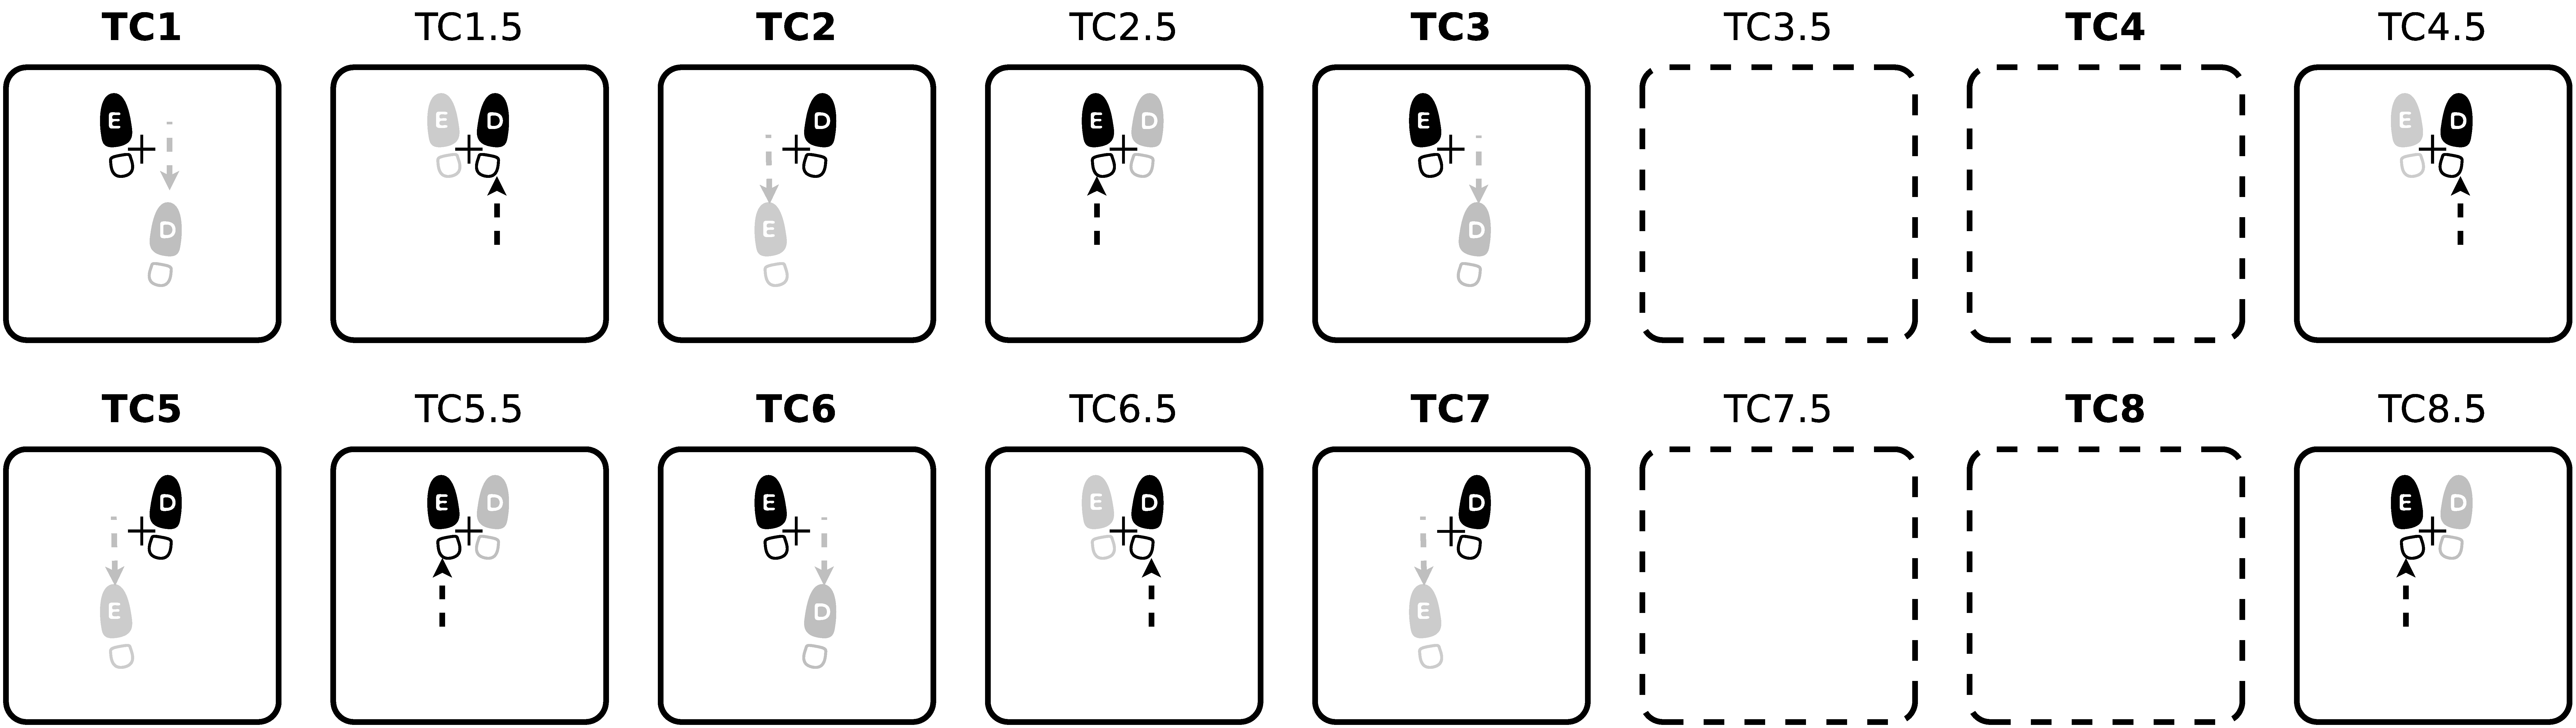
\includegraphics[width=\textwidth]{chapters/cap-passos-footwork/escovinha2tras.eps}
\caption{Diagrama detalhado de tempos coreográficos para a escovinha para atrás, $T=2~TC$.}
\label{fig:pessoalescovinha2tras}
\end{sidewaysfigure}



%%%%%%%%%%%%%%%%%%%%%%%%%%%%%%%%%%%%%%%%%%%%%%%%%%%%%%%%%%%%%%%%%%%%%%%%%%%%%%%%
\clearpage
\section{ \Variante: Escovinha trocando de lados}\index{Passo!Escovinha trocando de lados}


A Figura \ref{fig:pessoa-escovinha-ambos-lados} mostra os movimentos necessários para executar uma variante do passo chamado pica-pau.
\begin{itemize}
\item Cada quadro de trabalho representa a posição dos pés em cada tempo coreográfico;
\item um tempo coreográfico tem uma duração igual a meio tempo musical (T).
\item O passo básico de samba no pé  pode ser executado de forma cíclica, de modo que 
a sequencia de passos pode executar-se como: TC1, TC2, ..., TC7, TC8, TC1, TC2, ..., etc.  
Quantas vesses se considere necessário.
\end{itemize}

\begin{figure}[!h]
  \centering
    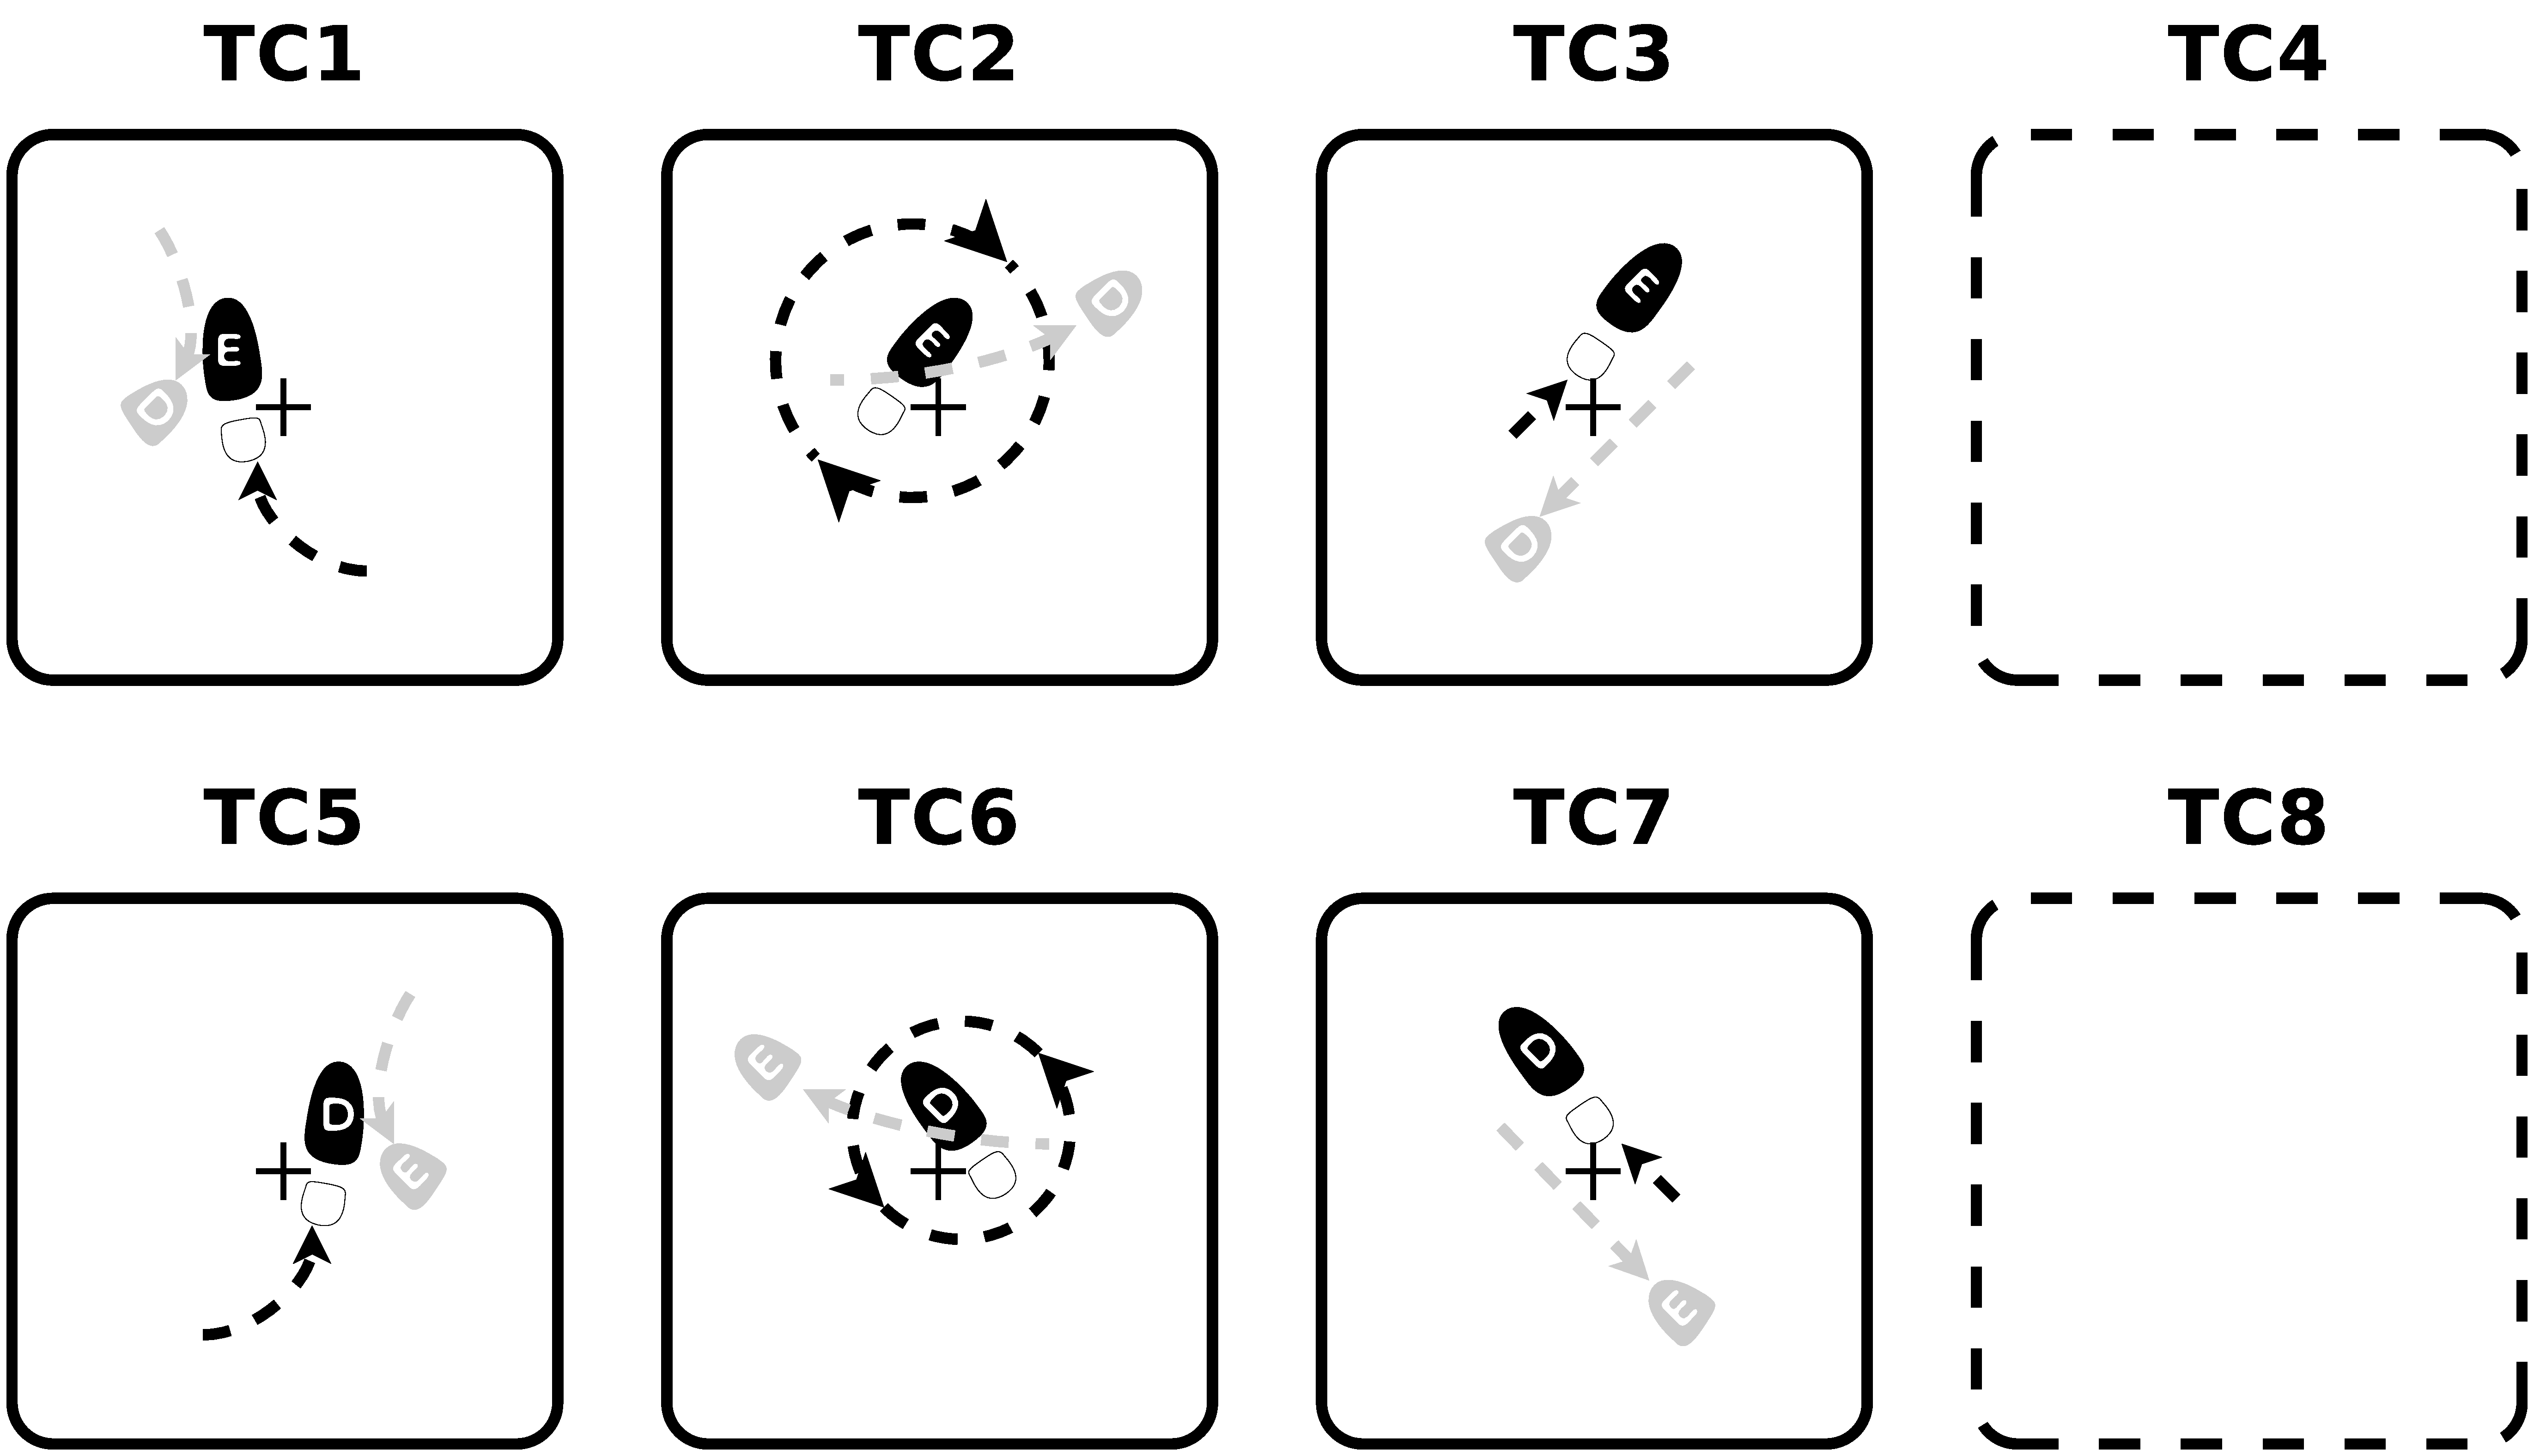
\includegraphics[width=\workboxsize]{chapters/cap-passos-footwork/escovinha-ambos-lados.eps}
\caption{Diagrama de tempos coreográficos para o passo escovinha intercambiando lados, $T=2~TC$.}
\label{fig:pessoa-escovinha-ambos-lados}
\end{figure}


A Figura \ref{fig:abc-pessoal-escovinha-ambos-lados} mostra o diagrama de tempos coreográficos para realizar o passo escovinha intercambiando lados,
explicada na Figura \ref{fig:pessoa-escovinha-ambos-lados}.

\begin{figure}[!h]
  \centering
\begin{abc}[name=abc-pessoal-escovinha-ambos-lados,width=0.7\linewidth]
X: 1 % start of header
K: C stafflines=1 % scale: C major
M: 2/4 %meter - compasso
%Q:1/4=80
V:1 clef=perc stem=up name="Ritmo" sname="Ritmo"
V:2 clef=perc stem=up name="TC"    sname="TC"
[V:1] |: B2  B1  B1 | B2  B1  B1 :| 
w:       ~  tchic tchic tum tchic tchic 
w: tum ~ ~ ~ ~ ~ 
w: ~ ~ ~ ~ ~ ~ 
[V:2] |: B2  B1  B1 | B2  B1  B1 :| 
w:       ~   TC1 TC2  TC3 TC5 TC6 
w:       TC7  
\end{abc}
\caption{Diagrama de tempos para a execução do passo escovinha intercambiando lados.}
\label{fig:abc-pessoal-escovinha-ambos-lados}
\end{figure}


%%%%%%%%%%%%%%%%%%%%%%%%%%%%%%%%%%%%%%%%%%%%%%%%%%%%%%%%%%%%%%%%%%%%%%%%%%%%%%%%
\begin{comment}
\section{\textcolor{red}{\Variante: Pescaria}}\index{Passo!Pescaria}
\end{comment}

%%%%%%%%%%%%%%%%%%%%%%%%%%%%%%%%%%%%%%%%%%%%%%%%%%%%%%%%%%%%%%%%%%%%%%%%%%%%%%%%
\begin{comment}
\section{\textcolor{red}{\Variante: Puladinho}}\index{Passo!Puladinho}
\end{comment}

